\documentclass[parskip]{scrartcl}
\usepackage{tikz}
\usepackage{pifont}
\usepackage{anttor}
\usepackage{ifsym}
\usepackage[utf8]{inputenc}
%\usepackage{fontawesome}
\usepackage{fontawesome5}
\usepackage[top=1cm,bottom=2cm,left=0.3cm,right=0.3cm]{geometry}
\usepackage{fancyhdr}
\graphicspath{ {./images/} }

\definecolor{apricot}{HTML}{F5B041}
\definecolor{lightblue}{HTML}{7FB3D5}
\definecolor{lightgreen}{HTML}{58D68D}
\definecolor{darkpink}{HTML}{AD1457}

\renewcommand\headrulewidth{0pt}   
\renewcommand\footrulewidth{0pt} 
\fancyfoot[RO,RE]{\textit{von Gabriela Brüll und Alexandra Mauel}}
\begin{document}
	\pgfmathsetmacro{\cardwidth}{5}
	\pgfmathsetmacro{\cardheight}{8}
	\pgfmathsetmacro{\stripwidth}{0.6}
	\pgfmathsetmacro{\strippadding}{0.1}
	\pgfmathsetmacro{\textpadding}{0.1}
	\pgfmathsetmacro{\ruleheight}{0.15}
%-------------------------------
%----Information zum Druck------
%-------------------------------
\vspace{-0.5cm}\pagestyle{fancy}
\textcolor{darkpink}{\textbf{Anmerkungen zum Druck:}} Einseitig drucken und Vorder- und Rückseiten der Karten bzw. Anleitung zusammenkleben (evtl. auf Pappe). Die Karten unter ,,Lösung'' sind als Kontrolle (nicht zum Ausschneiden) gedacht.\\
\vspace{-0.2cm}\\
%-----------------------------------
%-------- PINK DECK --------------
%-----------------------------------
%
%----Interphase
\begin{tikzpicture}
	\draw[rounded corners=0.2cm] (0,0) rectangle (\cardwidth,\cardheight);
	\fill[pink,rounded corners=0.1cm] (\strippadding,\strippadding) rectangle (\strippadding+\stripwidth,\cardheight-\strippadding) node[rotate=90,above left,black,font=\large] {UNTER DEM MIKROSKOP\hspace{3pt}   \rotatebox[origin=c]{-90}{\faMicroscope}};
	\node[text width=(\cardwidth-\strippadding-\stripwidth-2*\textpadding-0.3)*1cm,below right] at (\strippadding+\stripwidth+\textpadding,\cardheight-\textpadding) {
		{\Large  }\\
		\vspace{0.7cm}
		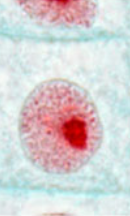
\includegraphics[width=\linewidth]{p/interphase}
	};
\end{tikzpicture}\hspace{1pt}
%----Prophase
\begin{tikzpicture}
	\draw[rounded corners=0.2cm] (0,0) rectangle (\cardwidth,\cardheight);
	\fill[pink,rounded corners=0.1cm] (\strippadding,\strippadding) rectangle (\strippadding+\stripwidth,\cardheight-\strippadding) node[rotate=90,above left,black,font=\large] {UNTER DEM MIKROSKOP\hspace{3pt}  \rotatebox[origin=c]{-90}{\faMicroscope}};
	\node[text width=(\cardwidth-\strippadding-\stripwidth-2*\textpadding-0.3)*1cm,below right] at (\strippadding+\stripwidth+\textpadding,\cardheight-\textpadding) {
		{\Large  }\\
		\vspace{0.7cm}
		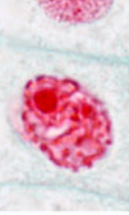
\includegraphics[width=\linewidth]{p/prophase}
	};
\end{tikzpicture}\hspace{1pt}
%----späte Prophase
\begin{tikzpicture}
	\draw[rounded corners=0.2cm] (0,0) rectangle (\cardwidth,\cardheight);
	\fill[pink,rounded corners=0.1cm] (\strippadding,\strippadding) rectangle (\strippadding+\stripwidth,\cardheight-\strippadding) node[rotate=90,above left,black,font=\large] {UNTER DEM MIKROSKOP\hspace{3pt} \rotatebox[origin=c]{-90}{\faMicroscope}};
	\node[text width=(\cardwidth-\strippadding-\stripwidth-2*\textpadding-0.3)*1cm,below right] at (\strippadding+\stripwidth+\textpadding,\cardheight-\textpadding) {
		{\Large  }\\
		\vspace{0.7cm}
		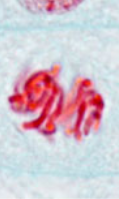
\includegraphics[width=\linewidth]{p/prophase2}
	};
\end{tikzpicture}\hspace{1pt}
%----Metaphase
\begin{tikzpicture}
\draw[rounded corners=0.2cm] (0,0) rectangle (\cardwidth,\cardheight);
\fill[pink,rounded corners=0.1cm] (\strippadding,\strippadding) rectangle (\strippadding+\stripwidth,\cardheight-\strippadding) node[rotate=90,above left,black,font=\large] {UNTER DEM MIKROSKOP\hspace{3pt} \rotatebox[origin=c]{-90}{\faMicroscope}};
\node[text width=(\cardwidth-\strippadding-\stripwidth-2*\textpadding-0.3)*1cm,below right] at (\strippadding+\stripwidth+\textpadding,\cardheight-\textpadding) {
	{\Large  }\\
	\vspace{0.7cm}
	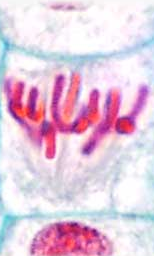
\includegraphics[width=\linewidth]{p/metaphase}
};
\end{tikzpicture}

%----späte Metaphase
\begin{tikzpicture}
	\draw[rounded corners=0.2cm] (0,0) rectangle (\cardwidth,\cardheight);
	\fill[pink,rounded corners=0.1cm] (\strippadding,\strippadding) rectangle (\strippadding+\stripwidth,\cardheight-\strippadding) node[rotate=90,above left,black,font=\large] {UNTER DEM MIKROSKOP \hspace{3pt}  \rotatebox[origin=c]{-90}{\faMicroscope}};
	\node[text width=(\cardwidth-\strippadding-\stripwidth-2*\textpadding-0.3)*1cm,below right] at (\strippadding+\stripwidth+\textpadding,\cardheight-\textpadding) {
		{\Large  }\\
		\vspace{0.7cm}
		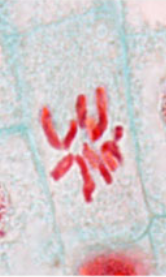
\includegraphics[width=\linewidth]{p/anaphase1}
	};
\end{tikzpicture}\hspace{1pt}
%----Anaphase
\begin{tikzpicture}
	\draw[rounded corners=0.2cm] (0,0) rectangle (\cardwidth,\cardheight);
	\fill[pink,rounded corners=0.1cm] (\strippadding,\strippadding) rectangle (\strippadding+\stripwidth,\cardheight-\strippadding) node[rotate=90,above left,black,font=\large] {UNTER DEM MIKROSKOP\hspace{3pt} \rotatebox[origin=c]{-90}{\faMicroscope}};
	\node[text width=(\cardwidth-\strippadding-\stripwidth-2*\textpadding-0.3)*1cm,below right] at (\strippadding+\stripwidth+\textpadding,\cardheight-\textpadding) {
		{\Large  }\\
		\vspace{0.7cm}
		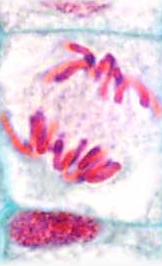
\includegraphics[width=\linewidth]{p/anaphase2}
	};
\end{tikzpicture}\hspace{1pt}
%----frühe Telophase
%\begin{tikzpicture}
%	\draw[rounded corners=0.2cm] (0,0) rectangle (\cardwidth,\cardheight);
%	\fill[pink,rounded corners=0.1cm] (\strippadding,\strippadding) rectangle (\strippadding+\stripwidth,\cardheight-\strippadding) node[rotate=90,above left,black,font=\large] {UNTER DEM MIKROSKOP  \rotatebox[origin=c]{-90}{\ding{172}}};
%	\node[text width=(\cardwidth-\strippadding-\stripwidth-2*\textpadding-0.3)*1cm,below right] at (\strippadding+\stripwidth+\textpadding,\cardheight-\textpadding) {
%		{\Large  }\\
%		\vspace{0.7cm}
%		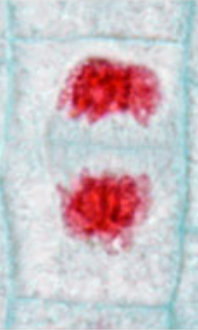
\includegraphics[width=\linewidth]{p/telophase1}
%	};
%\end{tikzpicture}
%
%
%----Telophase
\begin{tikzpicture}
	\draw[rounded corners=0.2cm] (0,0) rectangle (\cardwidth,\cardheight);
	\fill[pink,rounded corners=0.1cm] (\strippadding,\strippadding) rectangle (\strippadding+\stripwidth,\cardheight-\strippadding) node[rotate=90,above left,black,font=\large] {UNTER DEM MIKROSKOP\hspace{3pt}  \rotatebox[origin=c]{-90}{\faMicroscope}};
	\node[text width=(\cardwidth-\strippadding-\stripwidth-2*\textpadding-0.3)*1cm,below right] at (\strippadding+\stripwidth+\textpadding,\cardheight-\textpadding) {
		{\Large  }\\
		\vspace{0.7cm}
		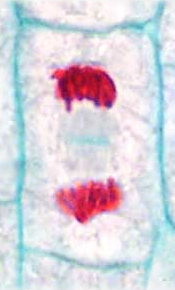
\includegraphics[width=\linewidth]{p/telophase2}
	};
\end{tikzpicture}\hspace{1pt}
%----Cytokinese
\begin{tikzpicture}
	\draw[rounded corners=0.2cm] (0,0) rectangle (\cardwidth,\cardheight);
	\fill[pink,rounded corners=0.1cm] (\strippadding,\strippadding) rectangle (\strippadding+\stripwidth,\cardheight-\strippadding) node[rotate=90,above left,black,font=\large] {UNTER DEM MIKROSKOP\hspace{3pt}  \rotatebox[origin=c]{-90}{\faMicroscope}};
	\node[text width=(\cardwidth-\strippadding-\stripwidth-2*\textpadding-0.3)*1cm,below right] at (\strippadding+\stripwidth+\textpadding,\cardheight-\textpadding) {
		{\Large  }\\
		\vspace{0.7cm}
		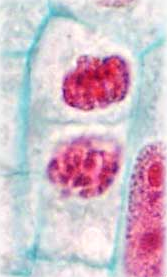
\includegraphics[width=\linewidth]{p/cytokinese}
	};
\end{tikzpicture}

%-----------------------------------
%-------- ORANGE DECK 1--------------
%-----------------------------------
%
%-------Interphase
%
\begin{tikzpicture}
	\draw[rounded corners=0.2cm] (0,0) rectangle (\cardwidth,\cardheight);
	\fill[apricot,rounded corners=0.1cm] (\strippadding,\strippadding) rectangle (\strippadding+\stripwidth,\cardheight-\strippadding) node[rotate=90,above left,black,font=\large] {ZEICHNUNG\hspace{3pt} \rotatebox[origin=c]{-90}{\footnotesize\faIcon[regular]{edit}}};
	\node[text width=(\cardwidth-\strippadding-\stripwidth-2*\textpadding-0.3)*1cm,below right] at (\strippadding+\stripwidth+\textpadding,\cardheight-\textpadding) {
		{\Large  }\\
		\vspace{1.1cm}
		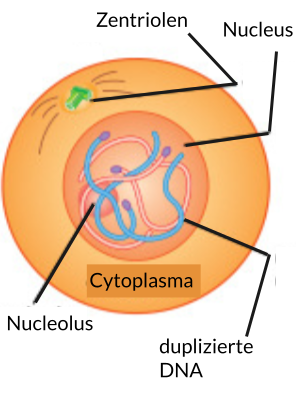
\includegraphics[width=\linewidth]{o/interphase}
	};
\end{tikzpicture}\hspace{1pt}
%
%-------Prophase
%
\begin{tikzpicture}
	\draw[rounded corners=0.2cm] (0,0) rectangle (\cardwidth,\cardheight);
	\fill[apricot,rounded corners=0.1cm] (\strippadding,\strippadding) rectangle (\strippadding+\stripwidth,\cardheight-\strippadding) node[rotate=90,above left,black,font=\large] { ZEICHNUNG\hspace{3pt}  \rotatebox[origin=c]{-90}{\footnotesize\faIcon[regular]{edit}}};
	\node[text width=(\cardwidth-\strippadding-\stripwidth-2*\textpadding-0.3)*1cm,below right] at (\strippadding+\stripwidth+\textpadding,\cardheight-\textpadding) {
		{\Large  }\\
		\vspace{1.3cm}
		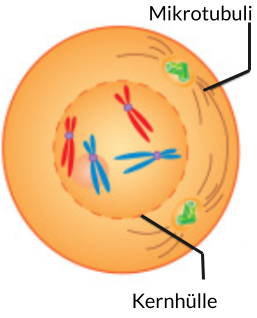
\includegraphics[width=\linewidth]{o/prophase}
	};
\end{tikzpicture}\hspace{1pt}
%
%-------Prometaphase
%
\begin{tikzpicture}
	\draw[rounded corners=0.2cm] (0,0) rectangle (\cardwidth,\cardheight);
	\fill[apricot,rounded corners=0.1cm] (\strippadding,\strippadding) rectangle (\strippadding+\stripwidth,\cardheight-\strippadding) node[rotate=90,above left,black,font=\large] { ZEICHNUNG\hspace{3pt}  \rotatebox[origin=c]{-90}{\footnotesize\faIcon[regular]{edit}}};
	\node[text width=(\cardwidth-\strippadding-\stripwidth-2*\textpadding-0.3)*1cm,below right] at (\strippadding+\stripwidth+\textpadding,\cardheight-\textpadding) {
		{\Large  }\\
		\vspace{1.3cm}
		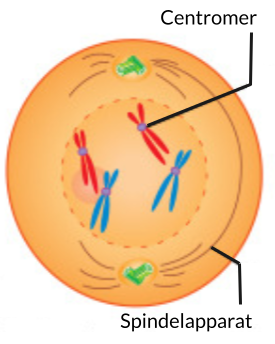
\includegraphics[width=\linewidth]{o/prometaphase}
	};
\end{tikzpicture}\hspace{1pt}
%
%-------Metaphase
%
\begin{tikzpicture}
	\draw[rounded corners=0.2cm] (0,0) rectangle (\cardwidth,\cardheight);
	\fill[apricot,rounded corners=0.1cm] (\strippadding,\strippadding) rectangle (\strippadding+\stripwidth,\cardheight-\strippadding) node[rotate=90,above left,black,font=\large] { ZEICHNUNG\hspace{3pt}  \rotatebox[origin=c]{-90}{\footnotesize\faIcon[regular]{edit}}};
	\node[text width=(\cardwidth-\strippadding-\stripwidth-2*\textpadding-0.3)*1cm,below right] at (\strippadding+\stripwidth+\textpadding,\cardheight-\textpadding) {
		{\Large  }\\
		\vspace{1.3cm}
		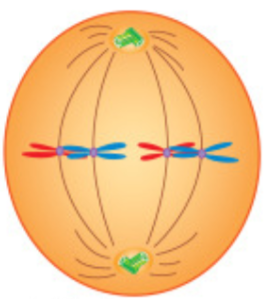
\includegraphics[width=\linewidth]{o/metaphase}
	};
\end{tikzpicture}
%-----------------------------------
%---------- BACK SIDE  -------------
%-----------------------------------
\begin{tikzpicture}
	\draw[rounded corners=0.2cm] (0,0) rectangle (\cardwidth,\cardheight);
	\node[text width=(\cardwidth-0.3)*1cm,below right] at (0,\cardheight+\textpadding) {
		{\Large  }\\
		\vspace{0.3cm}
		\hspace{3pt}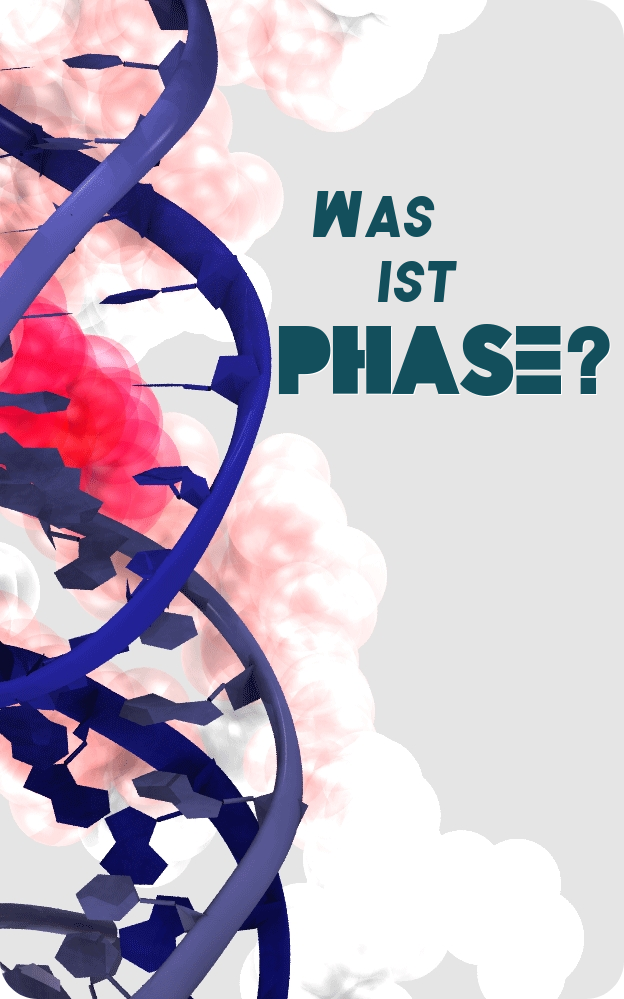
\includegraphics[width=0.95\linewidth]{back}
	};
\end{tikzpicture}\hspace{1pt}
\begin{tikzpicture}
	\draw[rounded corners=0.2cm] (0,0) rectangle (\cardwidth,\cardheight);
	\node[text width=(\cardwidth-0.3)*1cm,below right] at (0,\cardheight+\textpadding) {
		{\Large  }\\
		\vspace{0.3cm}
		\hspace{3pt}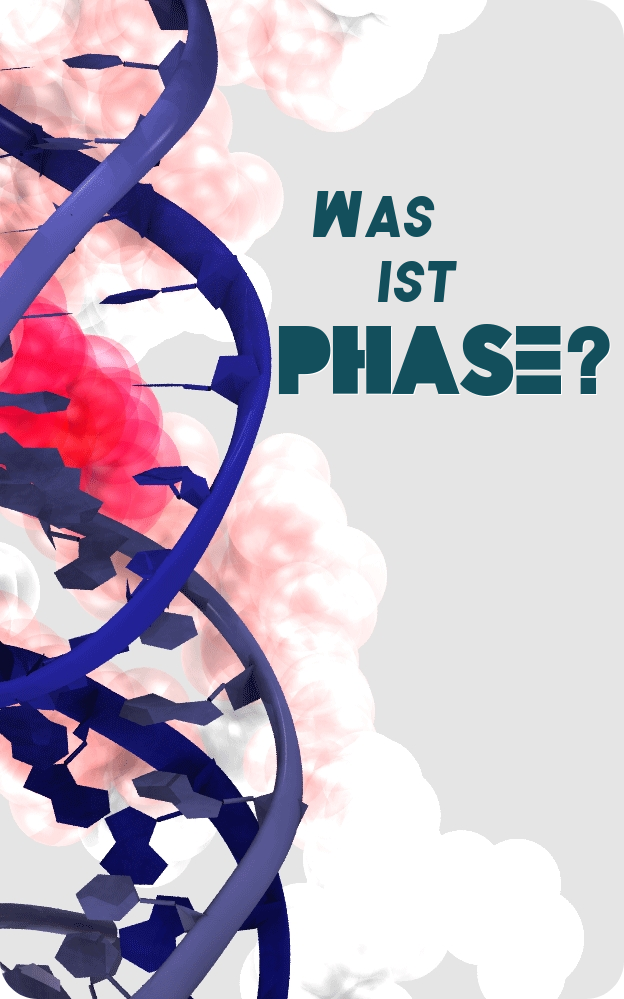
\includegraphics[width=0.95\linewidth]{back}
	};
\end{tikzpicture}\hspace{1pt}
\begin{tikzpicture}
	\draw[rounded corners=0.2cm] (0,0) rectangle (\cardwidth,\cardheight);
	\node[text width=(\cardwidth-0.3)*1cm,below right] at (0,\cardheight+\textpadding) {
		{\Large  }\\
		\vspace{0.3cm}
		\hspace{3pt}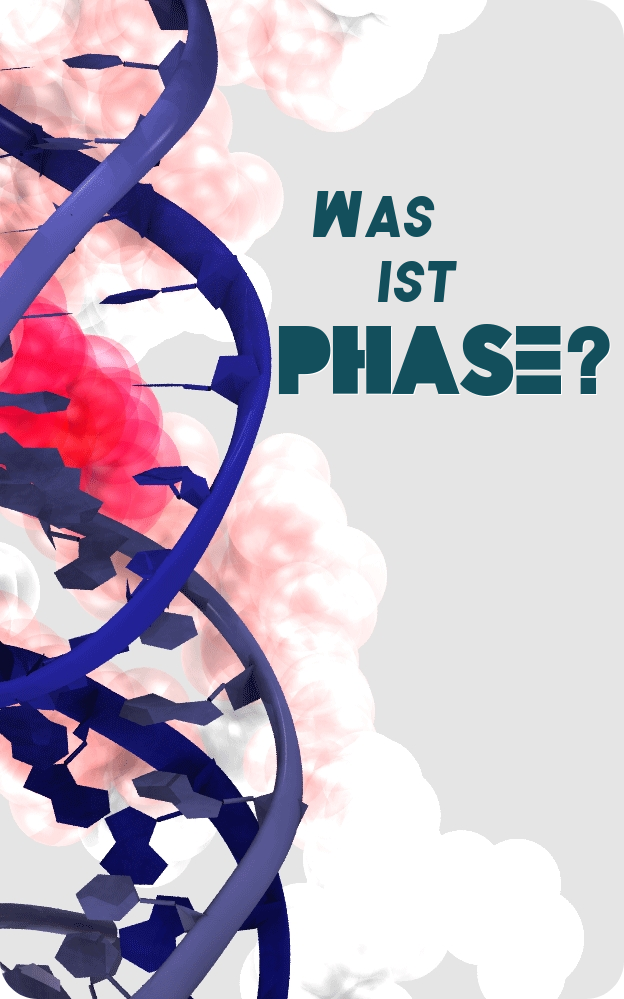
\includegraphics[width=0.95\linewidth]{back}
	};
\end{tikzpicture}\hspace{1pt}
\begin{tikzpicture}
	\draw[rounded corners=0.2cm] (0,0) rectangle (\cardwidth,\cardheight);
	\node[text width=(\cardwidth)*1cm,below right] at (0,\cardheight+\textpadding) {
		{\Large  }\\
		\vspace{0.3cm}
		\hspace{3pt}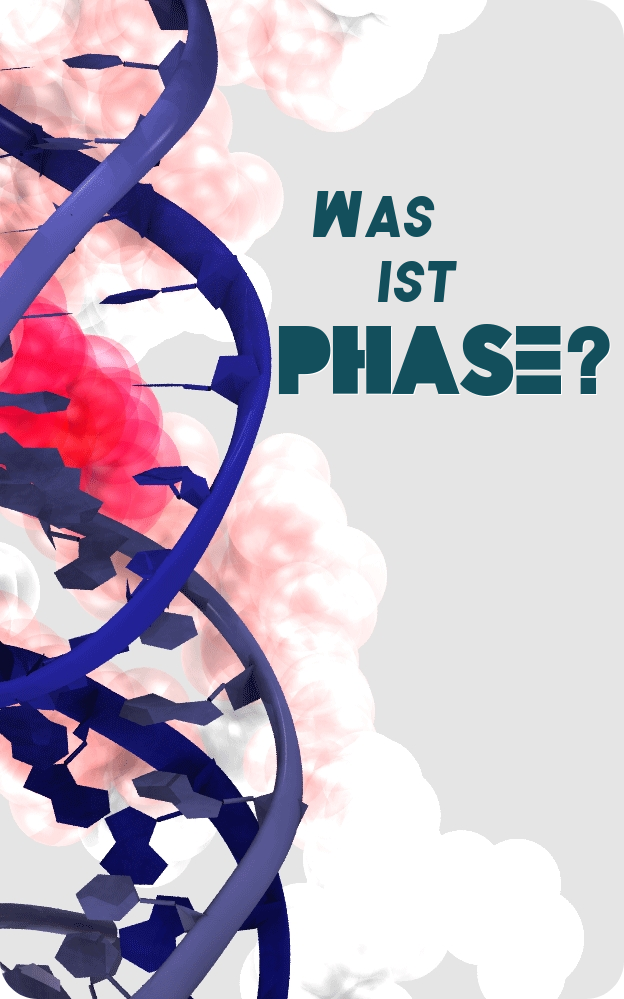
\includegraphics[width=.9\linewidth]{back}
	};
\end{tikzpicture}

\begin{tikzpicture}
	\draw[rounded corners=0.2cm] (0,0) rectangle (\cardwidth,\cardheight);
	\node[text width=(\cardwidth-0.3)*1cm,below right] at (0,\cardheight+\textpadding) {
		{\Large  }\\
		\vspace{0.3cm}
		\hspace{3pt}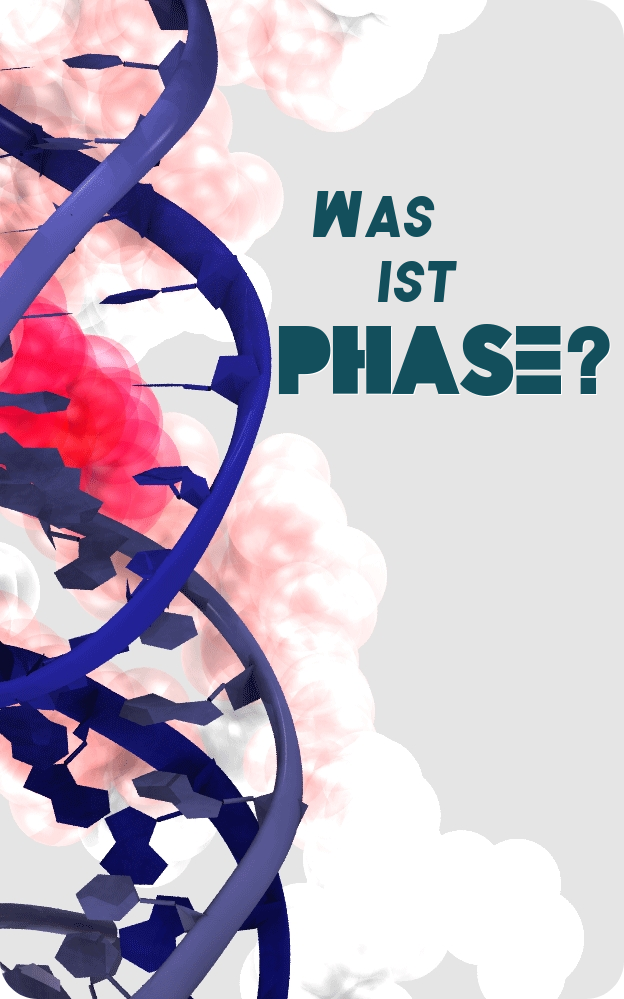
\includegraphics[width=0.95\linewidth]{back}
	};
\end{tikzpicture}\hspace{1pt}
\begin{tikzpicture}
	\draw[rounded corners=0.2cm] (0,0) rectangle (\cardwidth,\cardheight);
	\node[text width=(\cardwidth-0.3)*1cm,below right] at (0,\cardheight+\textpadding) {
		{\Large  }\\
		\vspace{0.3cm}
		\hspace{3pt}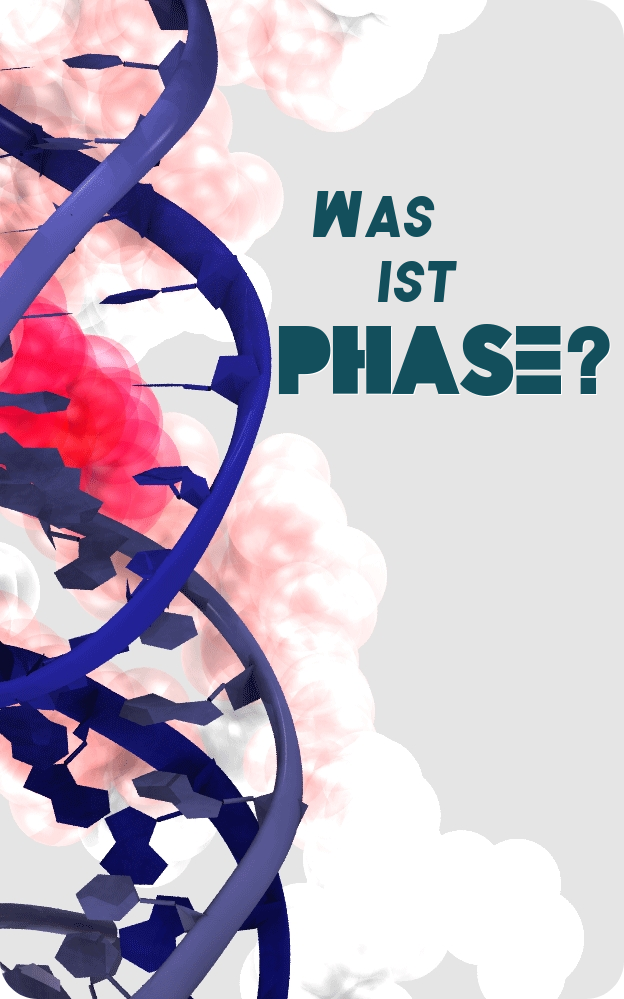
\includegraphics[width=0.95\linewidth]{back}
	};
\end{tikzpicture}\hspace{1pt}
\begin{tikzpicture}
	\draw[rounded corners=0.2cm] (0,0) rectangle (\cardwidth,\cardheight);
	\node[text width=(\cardwidth-0.3)*1cm,below right] at (0,\cardheight+\textpadding) {
		{\Large  }\\
		\vspace{0.3cm}
		\hspace{3pt}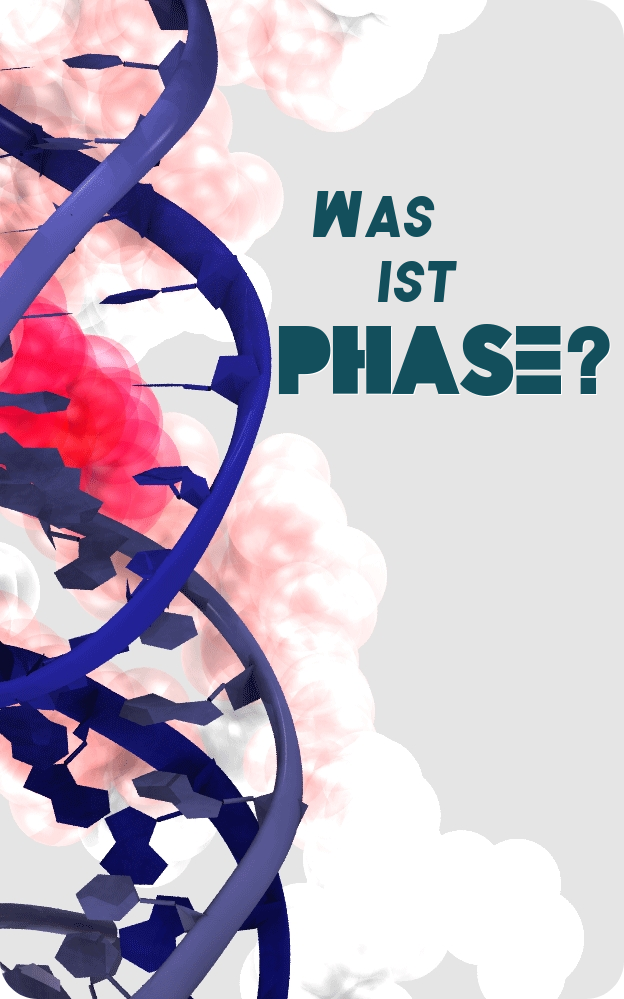
\includegraphics[width=0.95\linewidth]{back}
	};
\end{tikzpicture}\hspace{1pt}
\begin{tikzpicture}
	\draw[rounded corners=0.2cm] (0,0) rectangle (\cardwidth,\cardheight);
	\node[text width=(\cardwidth)*1cm,below right] at (0,\cardheight+\textpadding) {
		{\Large  }\\
		\vspace{0.3cm}
		\hspace{3pt}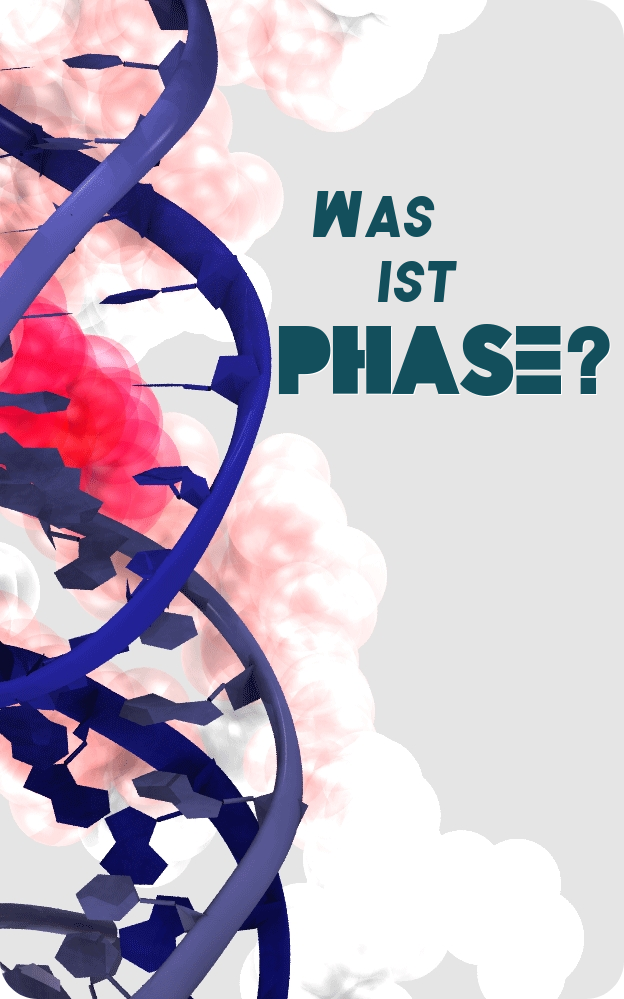
\includegraphics[width=.9\linewidth]{back}
	};
\end{tikzpicture}

\begin{tikzpicture}
	\draw[rounded corners=0.2cm] (0,0) rectangle (\cardwidth,\cardheight);
	\node[text width=(\cardwidth-0.3)*1cm,below right] at (0,\cardheight+\textpadding) {
		{\Large  }\\
		\vspace{0.3cm}
		\hspace{3pt}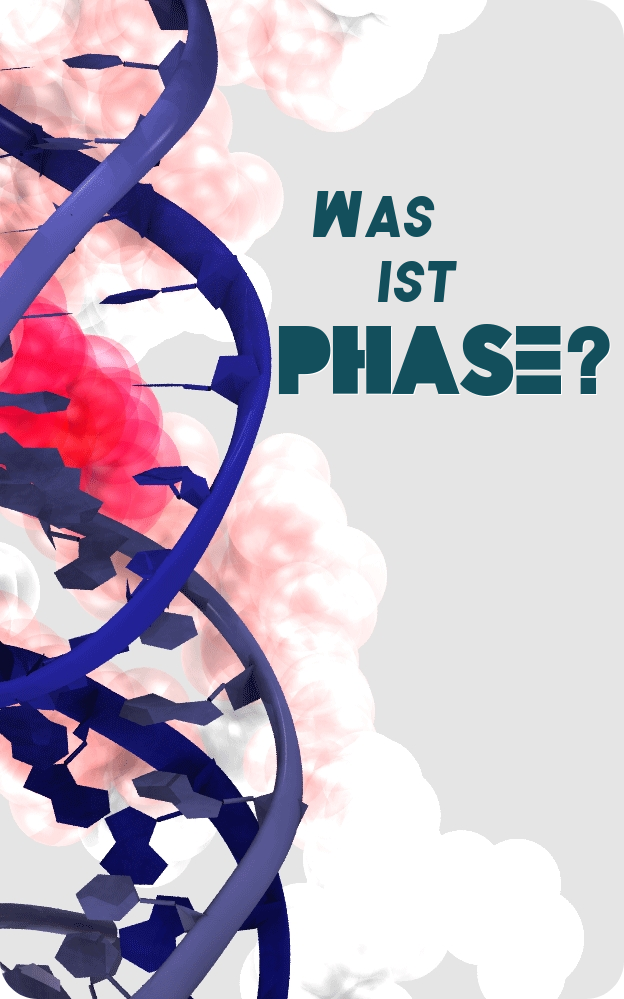
\includegraphics[width=0.95\linewidth]{back}
	};
\end{tikzpicture}\hspace{1pt}
\begin{tikzpicture}
	\draw[rounded corners=0.2cm] (0,0) rectangle (\cardwidth,\cardheight);
	\node[text width=(\cardwidth-0.3)*1cm,below right] at (0,\cardheight+\textpadding) {
		{\Large  }\\
		\vspace{0.3cm}
		\hspace{3pt}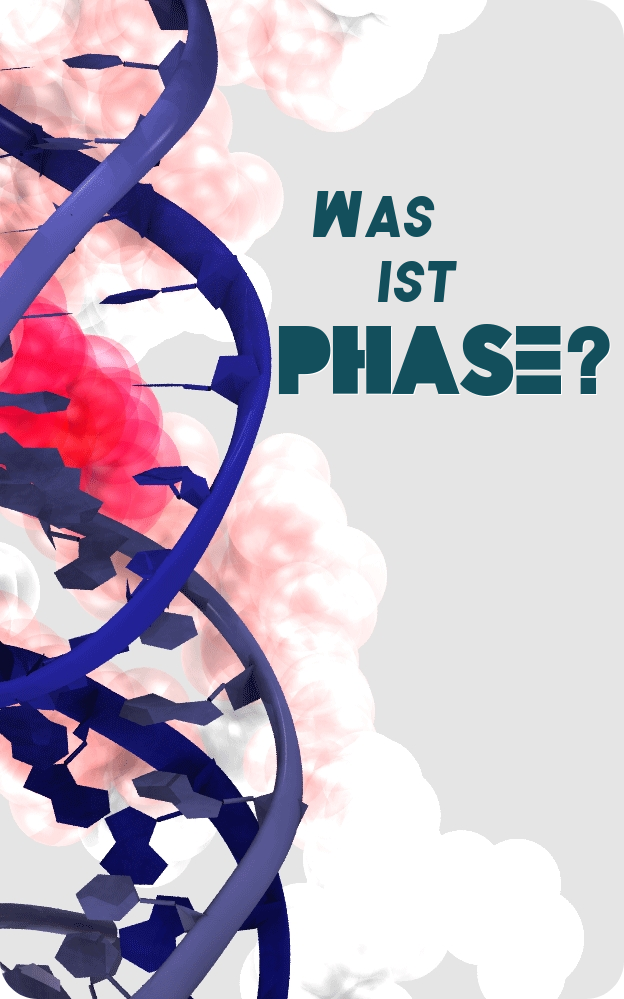
\includegraphics[width=0.95\linewidth]{back}
	};
\end{tikzpicture}\hspace{1pt}
\begin{tikzpicture}
	\draw[rounded corners=0.2cm] (0,0) rectangle (\cardwidth,\cardheight);
	\node[text width=(\cardwidth-0.3)*1cm,below right] at (0,\cardheight+\textpadding) {
		{\Large  }\\
		\vspace{0.3cm}
		\hspace{3pt}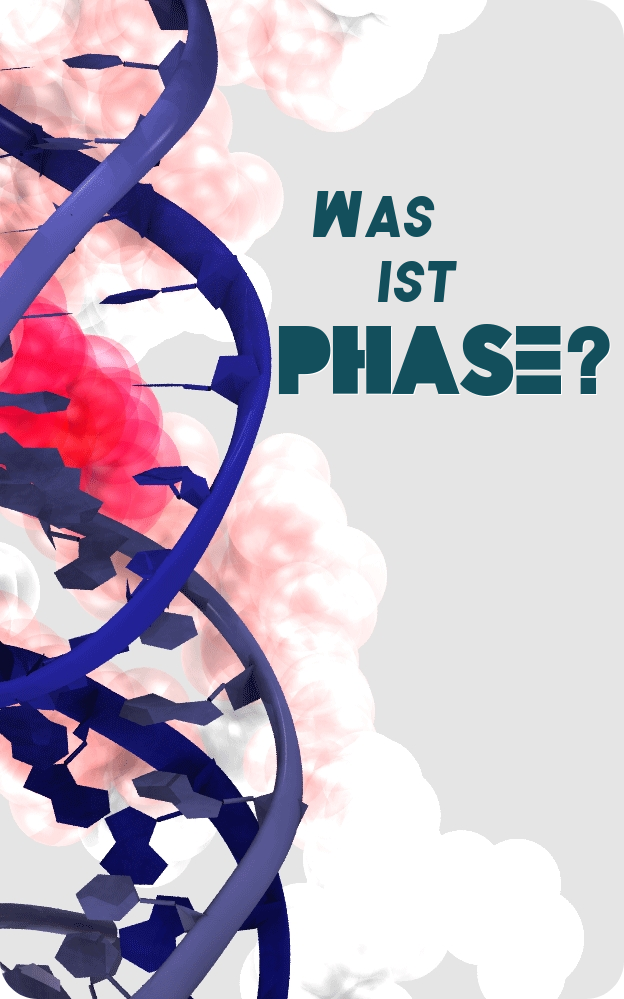
\includegraphics[width=0.95\linewidth]{back}
	};
\end{tikzpicture}\hspace{1pt}
\begin{tikzpicture}
	\draw[rounded corners=0.2cm] (0,0) rectangle (\cardwidth,\cardheight);
	\node[text width=(\cardwidth)*1cm,below right] at (0,\cardheight+\textpadding) {
		{\Large  }\\
		\vspace{0.3cm}
		\hspace{3pt}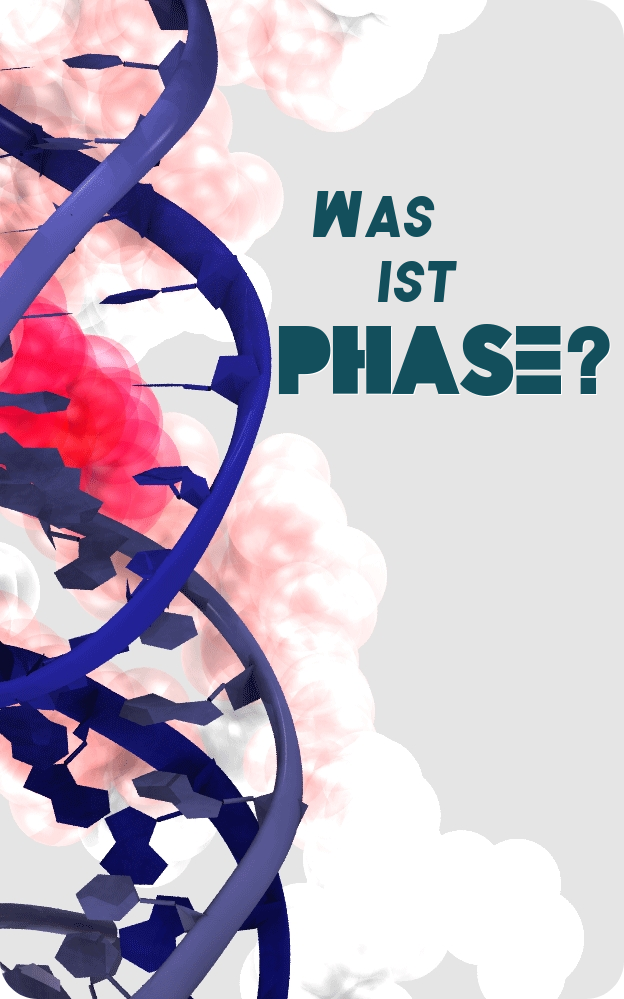
\includegraphics[width=.9\linewidth]{back}
	};
\end{tikzpicture}
%-----------------------------------
%-------- ORANGE DECK 2--------------
%-----------------------------------
%
%-------Anaphase
%
\begin{tikzpicture}
	\draw[rounded corners=0.2cm] (0,0) rectangle (\cardwidth,\cardheight);
	\fill[apricot,rounded corners=0.1cm] (\strippadding,\strippadding) rectangle (\strippadding+\stripwidth,\cardheight-\strippadding) node[rotate=90,above left,black,font=\large] { ZEICHNUNG\hspace{3pt}  \rotatebox[origin=c]{-90}{\footnotesize\faIcon[regular]{edit}}};
	\node[text width=(\cardwidth-\strippadding-\stripwidth-2*\textpadding-0.3)*1cm,below right] at (\strippadding+\stripwidth+\textpadding,\cardheight-\textpadding) {
		{\Large  }\\
		\vspace{1.3cm}
		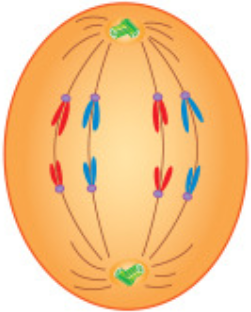
\includegraphics[width=\linewidth]{o/anaphase}
	};
\end{tikzpicture}\hspace{1pt}
%
%-------Telophase
%
\begin{tikzpicture}
	\draw[rounded corners=0.2cm] (0,0) rectangle (\cardwidth,\cardheight);
	\fill[apricot,rounded corners=0.1cm] (\strippadding,\strippadding) rectangle (\strippadding+\stripwidth,\cardheight-\strippadding) node[rotate=90,above left,black,font=\large] { ZEICHNUNG\hspace{3pt}  \rotatebox[origin=c]{-90}{\footnotesize\faIcon[regular]{edit}}};
	\node[text width=(\cardwidth-\strippadding-\stripwidth-2*\textpadding-0.3)*1cm,below right] at (\strippadding+\stripwidth+\textpadding,\cardheight-\textpadding) {
		{\Large  }\\
		\vspace{1cm}
		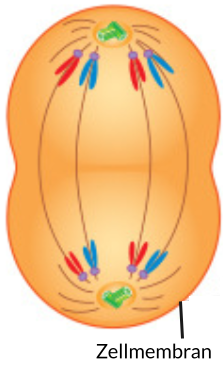
\includegraphics[width=\linewidth]{o/telophase}
	};
\end{tikzpicture}\hspace{1pt}
%
%-------späte Telophase
%
\begin{tikzpicture}
	\draw[rounded corners=0.2cm] (0,0) rectangle (\cardwidth,\cardheight);
	\fill[apricot,rounded corners=0.1cm] (\strippadding,\strippadding) rectangle (\strippadding+\stripwidth,\cardheight-\strippadding) node[rotate=90,above left,black,font=\large] { ZEICHNUNG\hspace{3pt}  \rotatebox[origin=c]{-90}{\footnotesize\faIcon[regular]{edit}}};
	\node[text width=(\cardwidth-\strippadding-\stripwidth-2*\textpadding-0.3)*1cm,below right] at (\strippadding+\stripwidth+\textpadding,\cardheight-\textpadding) {
		{\Large  }\\
		\vspace{1.3cm}
		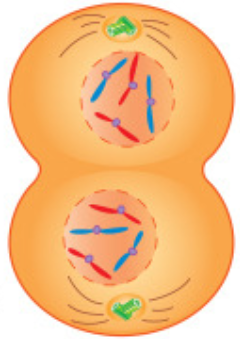
\includegraphics[width=\linewidth]{o/telophase2}
	};
\end{tikzpicture}\hspace{1pt}
%
%-------Cytokinese
%
\begin{tikzpicture}
	\draw[rounded corners=0.2cm] (0,0) rectangle (\cardwidth,\cardheight);
	\fill[apricot,rounded corners=0.1cm] (\strippadding,\strippadding) rectangle (\strippadding+\stripwidth,\cardheight-\strippadding) node[rotate=90,above left,black,font=\large] { ZEICHNUNG\hspace{3pt}  \rotatebox[origin=c]{-90}{\footnotesize\faIcon[regular]{edit}}};
	\node[text width=(\cardwidth-\strippadding-\stripwidth-2*\textpadding-0.3)*1cm,below right] at (\strippadding+\stripwidth+\textpadding,\cardheight-\textpadding) {
		{\Large  }\\
		\vspace{1.3cm}
		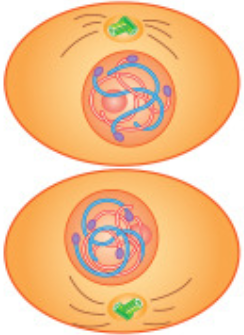
\includegraphics[width=\linewidth]{o/cytokinese}
	};
\end{tikzpicture}

%-----------------------------------
%---------- BLUE DECK --------------
%-----------------------------------
%
%-----Prophase
\begin{tikzpicture}
	\draw[rounded corners=0.2cm] (0,0) rectangle (\cardwidth,\cardheight);
	\fill[lightblue,rounded corners=0.1cm] (\strippadding,\strippadding) rectangle (\strippadding+\stripwidth,\cardheight-\strippadding) node[rotate=90,above left,black,font=\large] {BESCHREIBUNG\hspace{3pt}  \rotatebox[origin=c]{-90}{\faIcon[regular]{file-alt}}};
	\node[text width=(\cardwidth-\strippadding-\stripwidth-2*\textpadding-0.3)*1cm,below right] at (\strippadding+\stripwidth+\textpadding,\cardheight-\textpadding) {
		{\Large  }\\
		\vspace{0.6cm}
		{\scriptsize Das \textit{Chromatin} beginnt sich zu verdichten (kondensieren). Die \textit{Chromosomen} werden erkennbar. Jedes Chromosom besteht aus zwei identischen \textit{Chromatiden}, die über das \textit{Centromer} verbunden sind. Die Kernhülle und die Nucleoli lösen sich auf. Der \textit{Spindelapparat} bildet sich.}\\
	};
\end{tikzpicture}\hspace{1pt}
%-----Metaphase
\begin{tikzpicture}
	\draw[rounded corners=0.2cm] (0,0) rectangle (\cardwidth,\cardheight);
	\fill[lightblue,rounded corners=0.1cm] (\strippadding,\strippadding) rectangle (\strippadding+\stripwidth,\cardheight-\strippadding) node[rotate=90,above left,black,font=\large] {BESCHREIBUNG\hspace{3pt}  \rotatebox[origin=c]{-90}{\faIcon[regular]{file-alt}}};
	\node[text width=(\cardwidth-\strippadding-\stripwidth-2*\textpadding-0.3)*1cm,below right] at (\strippadding+\stripwidth+\textpadding,\cardheight-\textpadding) {
		{\Large  }\\
		\vspace{0.6cm}
		{\scriptsize Alle Chromosomen sind in der Zellmitte in einer Ebene, der \textit{Äquatorialplatte}, angeordnet. Man spricht auch von \textit{Metaphaseplatte}. Die \textit{Mikrotubuli} (Spindelfasern) des \textit{Spindelapparats} heften sich an die Centromere.}\\
	};
\end{tikzpicture}\hspace{1pt}
%-----Anaphase
\begin{tikzpicture}
	\draw[rounded corners=0.2cm] (0,0) rectangle (\cardwidth,\cardheight);
	\fill[lightblue,rounded corners=0.1cm] (\strippadding,\strippadding) rectangle (\strippadding+\stripwidth,\cardheight-\strippadding) node[rotate=90,above left,black,font=\large] {BESCHREIBUNG\hspace{3pt}  \rotatebox[origin=c]{-90}{\faIcon[regular]{file-alt}}};
	\node[text width=(\cardwidth-\strippadding-\stripwidth-2*\textpadding-0.3)*1cm,below right] at (\strippadding+\stripwidth+\textpadding,\cardheight-\textpadding) {
		{\Large  }\\
		\vspace{0.6cm}
		{\scriptsize Die \textit{Mikrotubuli} verkürzen sich, sodass sich die Verbindung der \textit{Schwesterchromatiden} am Centromer lösen und die \textit{Chromatiden} sich auf die entgegengesetzten Pole der Zelle zubewegen. }\\
	};
\end{tikzpicture}\hspace{1pt}
%-----Telophase
\begin{tikzpicture}
	\draw[rounded corners=0.2cm] (0,0) rectangle (\cardwidth,\cardheight);
	\fill[lightblue,rounded corners=0.1cm] (\strippadding,\strippadding) rectangle (\strippadding+\stripwidth,\cardheight-\strippadding) node[rotate=90,above left,black,font=\large] {BESCHREIBUNG\hspace{3pt}  \rotatebox[origin=c]{-90}{\faIcon[regular]{file-alt}}};
	\node[text width=(\cardwidth-\strippadding-\stripwidth-2*\textpadding-0.3)*1cm,below right] at (\strippadding+\stripwidth+\textpadding,\cardheight-\textpadding) {
		{\Large  }\\
		\vspace{0.6cm}
		{\scriptsize Die \textit{Chromatiden} sind an den Zellpolen angekommen. An jedem Pol liegt nun der vollständige diploide Satz \textit{Ein-Chromatid-Chromosomen} vor. Die Chromosomen entspiralisieren sich. Nucleoli und eine neue Kernmembran bilden sich aus. Die \textit{Mikrotubuli} werden abgebaut.}\\
	};
\end{tikzpicture}

%-----Cytokinese
\begin{tikzpicture}
	\draw[rounded corners=0.2cm] (0,0) rectangle (\cardwidth,\cardheight);
	\fill[lightblue,rounded corners=0.1cm] (\strippadding,\strippadding) rectangle (\strippadding+\stripwidth,\cardheight-\strippadding) node[rotate=90,above left,black,font=\large] {BESCHREIBUNG\hspace{3pt}  \rotatebox[origin=c]{-90}{\faIcon[regular]{file-alt}}};
	\node[text width=(\cardwidth-\strippadding-\stripwidth-2*\textpadding-0.3)*1cm,below right] at (\strippadding+\stripwidth+\textpadding,\cardheight-\textpadding) {
		{\Large  }\\
		\vspace{0.6cm}
		{\scriptsize Auf Höhe der ursprüng-lichen \textit{Äquatorialebene} bildet sich eine neue Zellmembran. Dieser Prozess startete bereits in der Telophase.}\\
	};
\end{tikzpicture}\hspace{1pt}
%-----Interphase G1
\begin{tikzpicture}
	\draw[rounded corners=0.2cm] (0,0) rectangle (\cardwidth,\cardheight);
	\fill[lightblue,rounded corners=0.1cm] (\strippadding,\strippadding) rectangle (\strippadding+\stripwidth,\cardheight-\strippadding) node[rotate=90,above left,black,font=\large] {BESCHREIBUNG\hspace{3pt}  \rotatebox[origin=c]{-90}{\faIcon[regular]{file-alt}}};
	\node[text width=(\cardwidth-\strippadding-\stripwidth-2*\textpadding-0.3)*1cm,below right] at (\strippadding+\stripwidth+\textpadding,\cardheight-\textpadding) {
		{\Large  }\\
		\vspace{0.6cm}
		{\scriptsize Die Zelle wächst. Die Bedingungen für eine Zellteilung werden überprüft. Sind diese gegeben, so bereitet sich die Zelle auf eine Verdopplung der \textit{Ein-Chromatid-Chromosomen} vor.}\\
	};
\end{tikzpicture}\hspace{1pt}
%----- Interphase S
\begin{tikzpicture}
	\draw[rounded corners=0.2cm] (0,0) rectangle (\cardwidth,\cardheight);
	\fill[lightblue,rounded corners=0.1cm] (\strippadding,\strippadding) rectangle (\strippadding+\stripwidth,\cardheight-\strippadding) node[rotate=90,above left,black,font=\large] {BESCHREIBUNG\hspace{3pt}  \rotatebox[origin=c]{-90}{\faIcon[regular]{file-alt}}};
	\node[text width=(\cardwidth-\strippadding-\stripwidth-2*\textpadding-0.3)*1cm,below right] at (\strippadding+\stripwidth+\textpadding,\cardheight-\textpadding) {
		{\Large  }\\
		\vspace{0.6cm}
		{\scriptsize Die Replikation der DNA beziehungsweise die Verdopplung der \textit{Chromatiden} findet statt.  Jedes \textit{Chromosom} besteht nun wieder aus zwei Chromatiden.}\\
	};
\end{tikzpicture}\hspace{1pt}
%-----Interphase G2
\begin{tikzpicture}
	\draw[rounded corners=0.2cm] (0,0) rectangle (\cardwidth,\cardheight);
	\fill[lightblue,rounded corners=0.1cm] (\strippadding,\strippadding) rectangle (\strippadding+\stripwidth,\cardheight-\strippadding) node[rotate=90,above left,black,font=\large] {BESCHREIBUNG\hspace{3pt}  \rotatebox[origin=c]{-90}{\faIcon[regular]{file-alt}}};
	\node[text width=(\cardwidth-\strippadding-\stripwidth-2*\textpadding-0.3)*1cm,below right] at (\strippadding+\stripwidth+\textpadding,\cardheight-\textpadding) {
		{\Large  }\\
		\vspace{0.6cm}
		{\scriptsize Die Vorbereitungen zur \textit{Kern-} und \textit{Zellteilung} werden abgeschlossen.}\\
	};
\end{tikzpicture}
%-----------------------------------
%---------- BACK SIDE  -------------
%-----------------------------------
\begin{tikzpicture}
	\draw[rounded corners=0.2cm] (0,0) rectangle (\cardwidth,\cardheight);
	\node[text width=(\cardwidth-0.3)*1cm,below right] at (0,\cardheight+\textpadding) {
		{\Large  }\\
		\vspace{0.3cm}
		\hspace{3pt}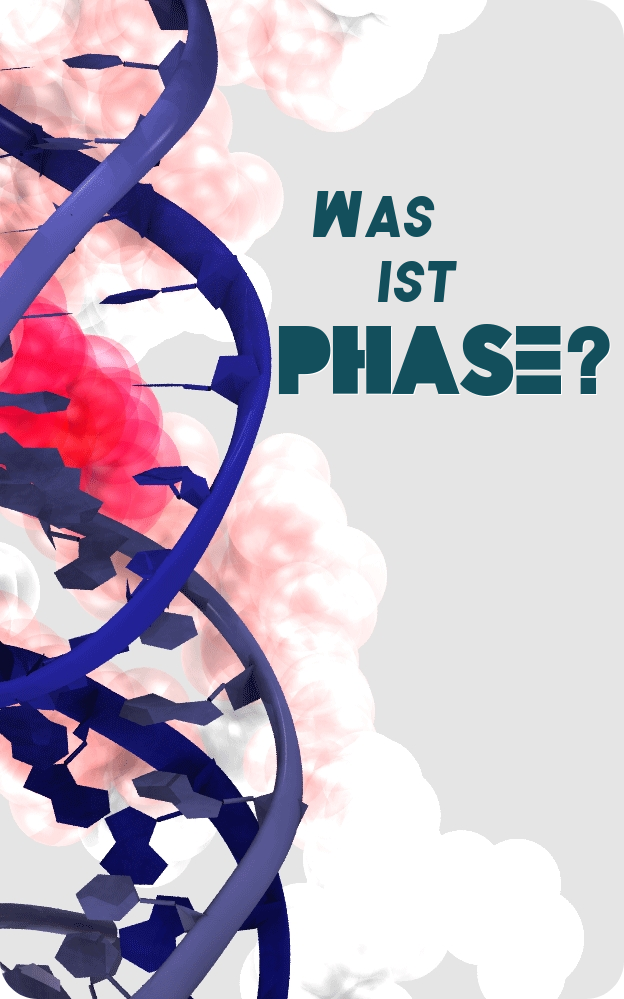
\includegraphics[width=0.95\linewidth]{back}
	};
\end{tikzpicture}\hspace{1pt}
\begin{tikzpicture}
	\draw[rounded corners=0.2cm] (0,0) rectangle (\cardwidth,\cardheight);
	\node[text width=(\cardwidth-0.3)*1cm,below right] at (0,\cardheight+\textpadding) {
		{\Large  }\\
		\vspace{0.3cm}
		\hspace{3pt}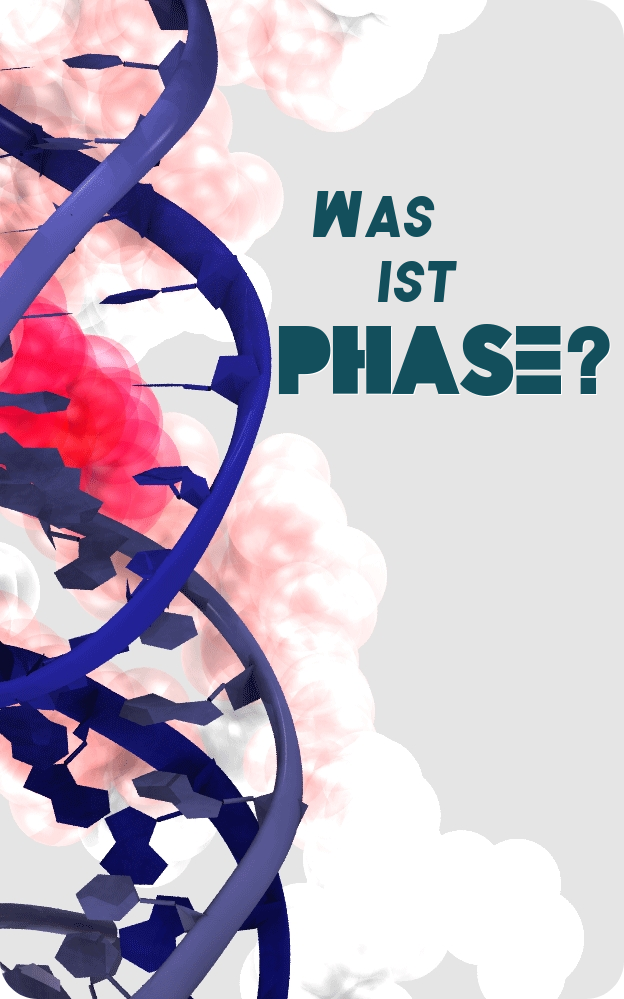
\includegraphics[width=0.95\linewidth]{back}
	};
\end{tikzpicture}\hspace{1pt}
\begin{tikzpicture}
	\draw[rounded corners=0.2cm] (0,0) rectangle (\cardwidth,\cardheight);
	\node[text width=(\cardwidth-0.3)*1cm,below right] at (0,\cardheight+\textpadding) {
		{\Large  }\\
		\vspace{0.3cm}
		\hspace{3pt}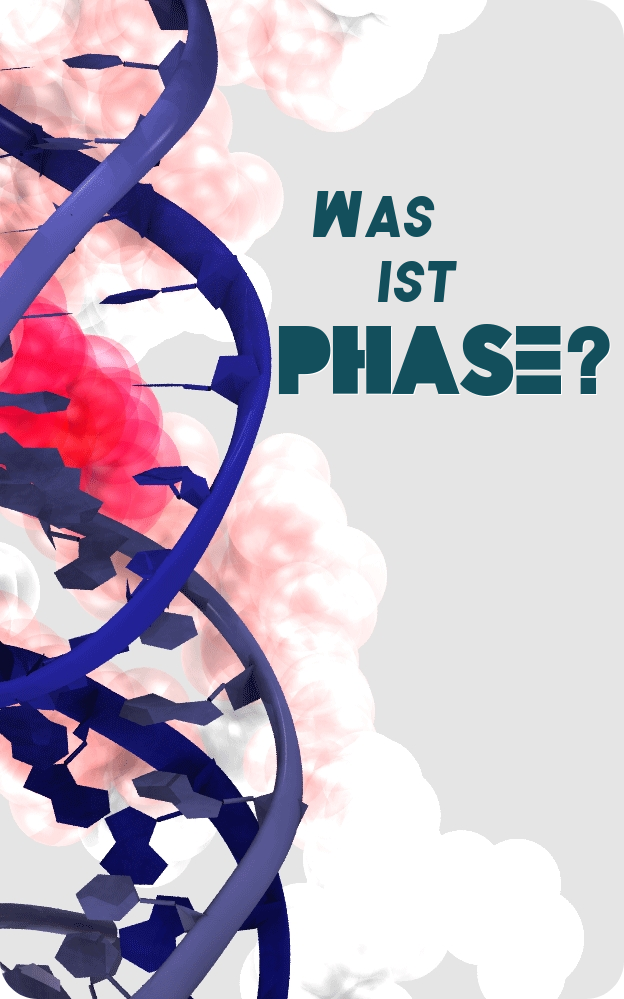
\includegraphics[width=0.95\linewidth]{back}
	};
\end{tikzpicture}\hspace{1pt}
\begin{tikzpicture}
	\draw[rounded corners=0.2cm] (0,0) rectangle (\cardwidth,\cardheight);
	\node[text width=(\cardwidth)*1cm,below right] at (0,\cardheight+\textpadding) {
		{\Large  }\\
		\vspace{0.3cm}
		\hspace{3pt}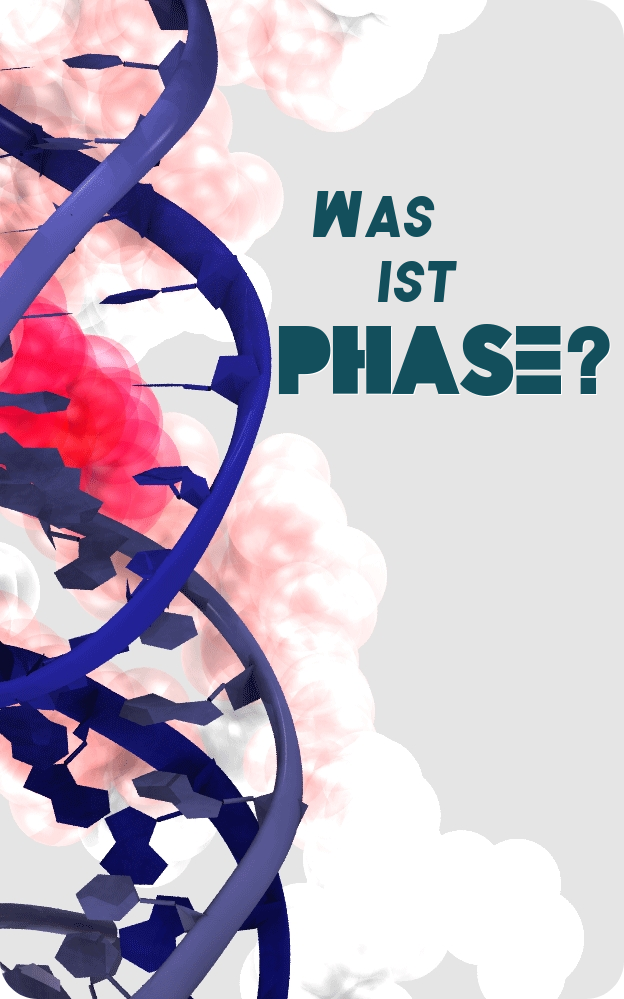
\includegraphics[width=.9\linewidth]{back}
	};
\end{tikzpicture}

\begin{tikzpicture}
	\draw[rounded corners=0.2cm] (0,0) rectangle (\cardwidth,\cardheight);
	\node[text width=(\cardwidth-0.3)*1cm,below right] at (0,\cardheight+\textpadding) {
		{\Large  }\\
		\vspace{0.3cm}
		\hspace{3pt}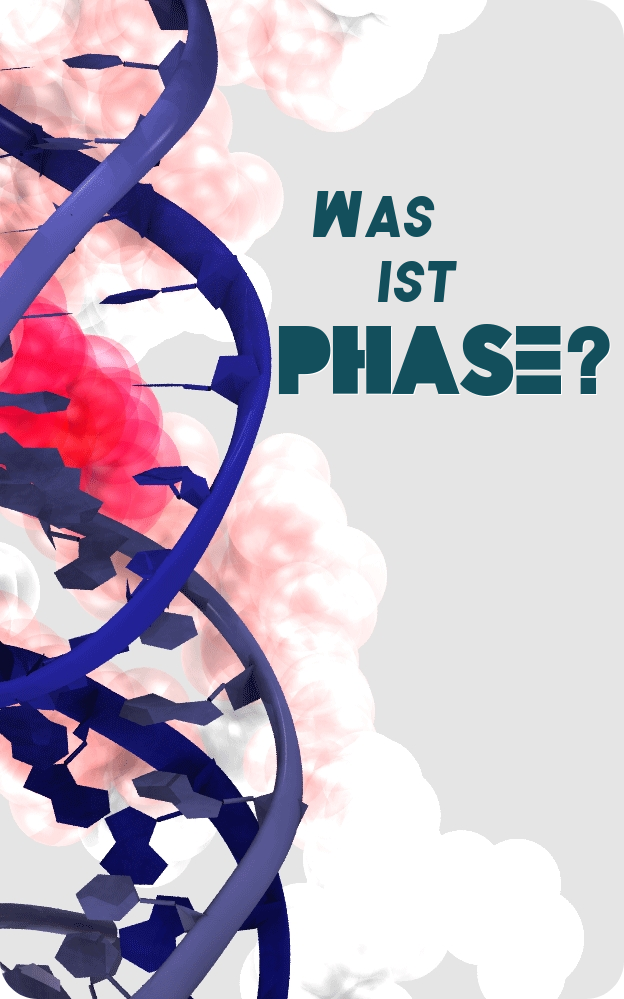
\includegraphics[width=0.95\linewidth]{back}
	};
\end{tikzpicture}\hspace{1pt}
\begin{tikzpicture}
	\draw[rounded corners=0.2cm] (0,0) rectangle (\cardwidth,\cardheight);
	\node[text width=(\cardwidth-0.3)*1cm,below right] at (0,\cardheight+\textpadding) {
		{\Large  }\\
		\vspace{0.3cm}
		\hspace{3pt}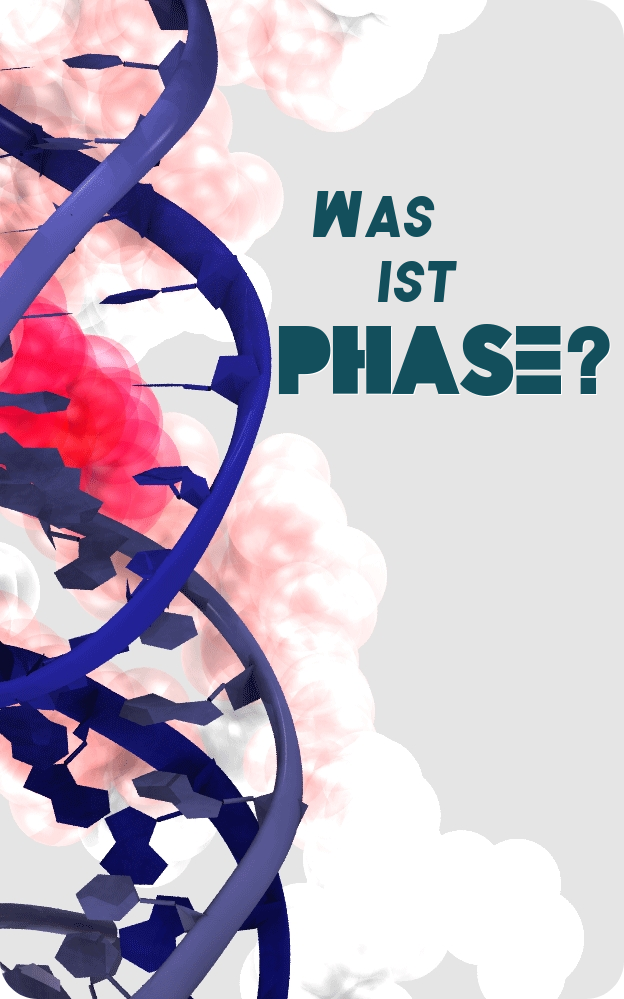
\includegraphics[width=0.95\linewidth]{back}
	};
\end{tikzpicture}\hspace{1pt}
\begin{tikzpicture}
	\draw[rounded corners=0.2cm] (0,0) rectangle (\cardwidth,\cardheight);
	\node[text width=(\cardwidth-0.3)*1cm,below right] at (0,\cardheight+\textpadding) {
		{\Large  }\\
		\vspace{0.3cm}
		\hspace{3pt}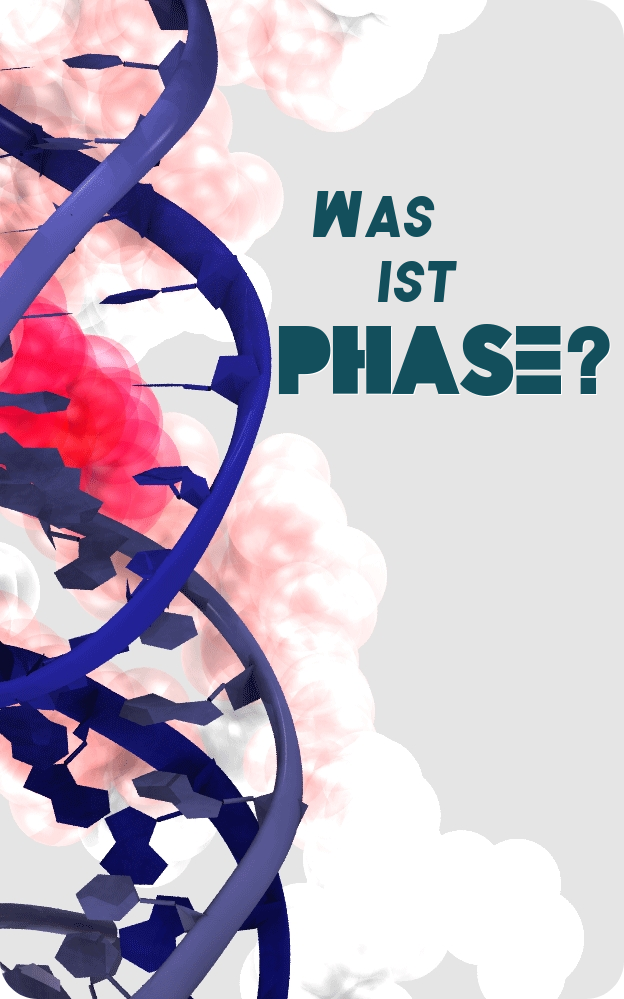
\includegraphics[width=0.95\linewidth]{back}
	};
\end{tikzpicture}\hspace{1pt}
\begin{tikzpicture}
	\draw[rounded corners=0.2cm] (0,0) rectangle (\cardwidth,\cardheight);
	\node[text width=(\cardwidth)*1cm,below right] at (0,\cardheight+\textpadding) {
		{\Large  }\\
		\vspace{0.3cm}
		\hspace{3pt}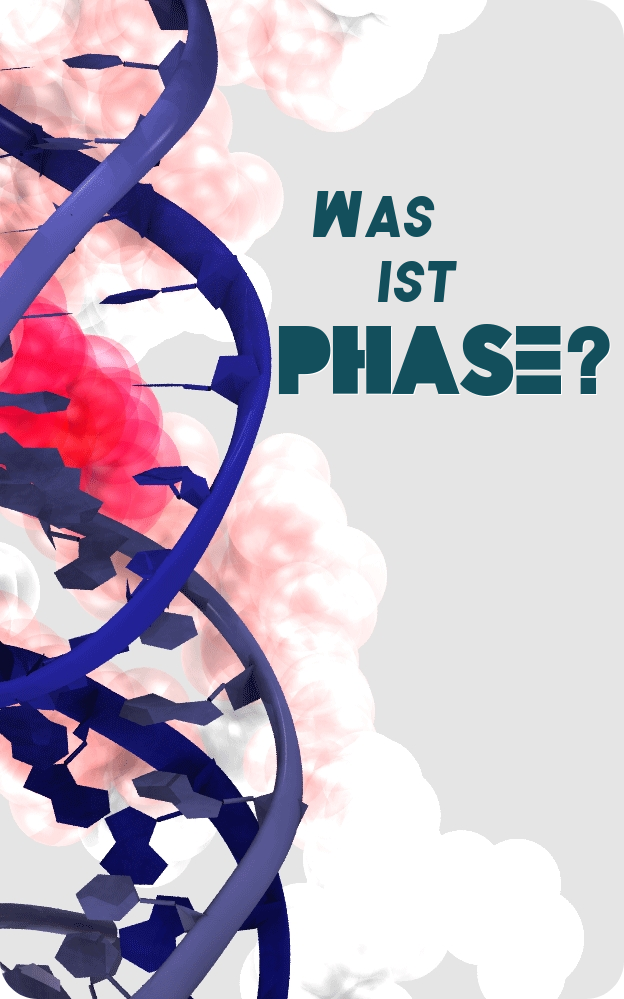
\includegraphics[width=.9\linewidth]{back}
	};
\end{tikzpicture}

\begin{tikzpicture}
	\draw[rounded corners=0.2cm] (0,0) rectangle (\cardwidth,\cardheight);
	\node[text width=(\cardwidth-0.3)*1cm,below right] at (0,\cardheight+\textpadding) {
		{\Large  }\\
		\vspace{0.3cm}
		\hspace{3pt}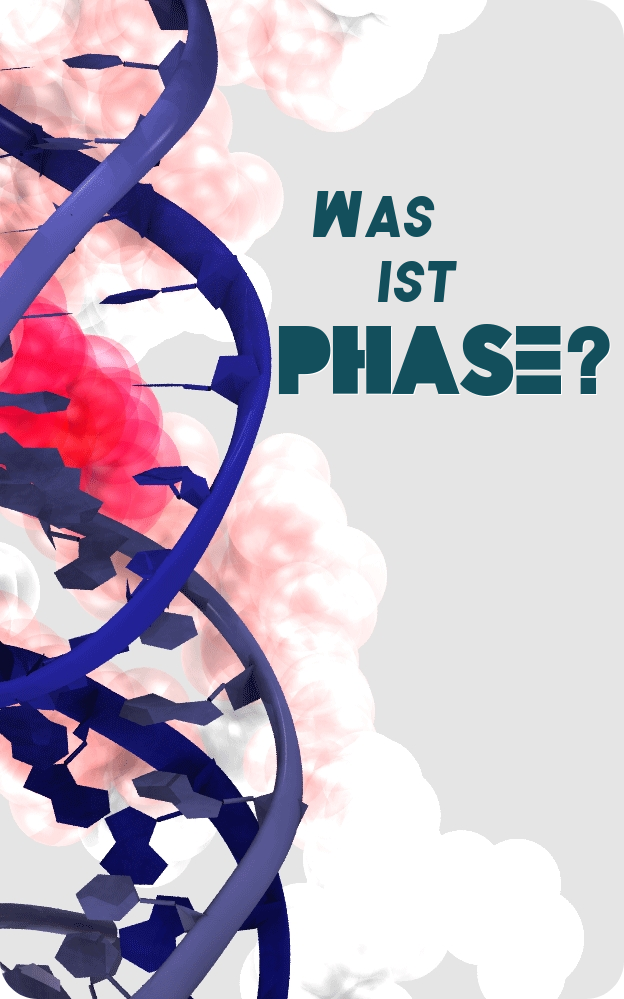
\includegraphics[width=0.95\linewidth]{back}
	};
\end{tikzpicture}\hspace{1pt}
\begin{tikzpicture}
	\draw[rounded corners=0.2cm] (0,0) rectangle (\cardwidth,\cardheight);
	\node[text width=(\cardwidth-0.3)*1cm,below right] at (0,\cardheight+\textpadding) {
		{\Large  }\\
		\vspace{0.3cm}
		\hspace{3pt}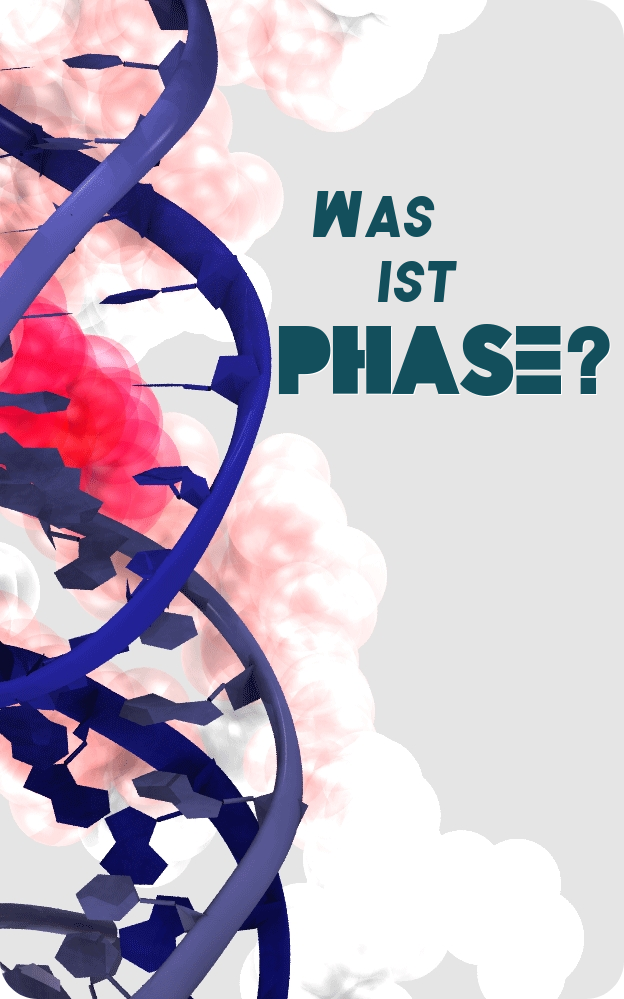
\includegraphics[width=0.95\linewidth]{back}
	};
\end{tikzpicture}\hspace{1pt}
\begin{tikzpicture}
	\draw[rounded corners=0.2cm] (0,0) rectangle (\cardwidth,\cardheight);
	\node[text width=(\cardwidth-0.3)*1cm,below right] at (0,\cardheight+\textpadding) {
		{\Large  }\\
		\vspace{0.3cm}
		\hspace{3pt}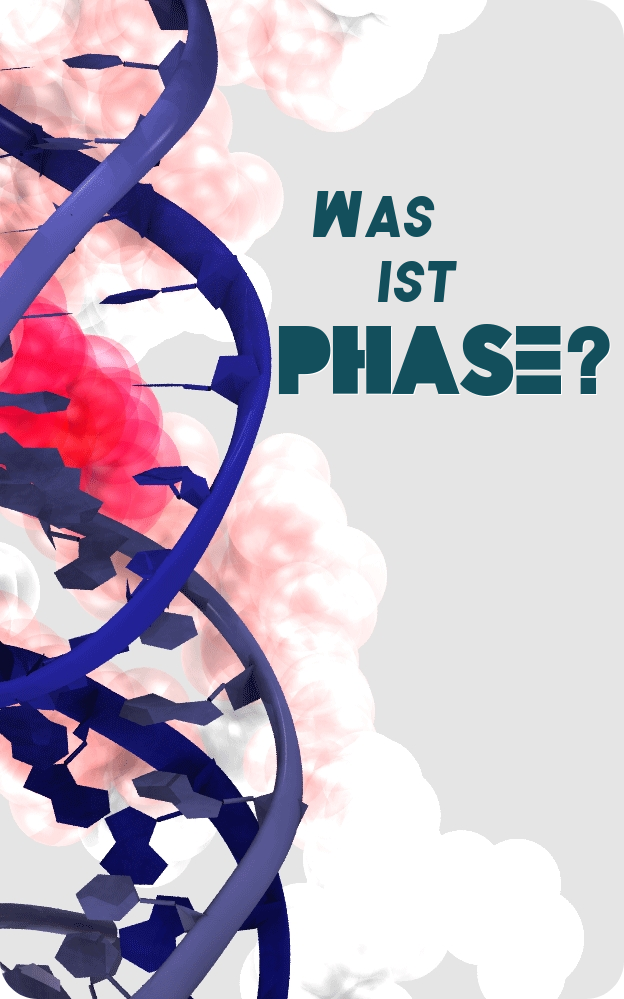
\includegraphics[width=0.95\linewidth]{back}
	};
\end{tikzpicture}\hspace{1pt}
\begin{tikzpicture}
	\draw[rounded corners=0.2cm] (0,0) rectangle (\cardwidth,\cardheight);
	\node[text width=(\cardwidth)*1cm,below right] at (0,\cardheight+\textpadding) {
		{\Large  }\\
		\vspace{0.3cm}
		\hspace{3pt}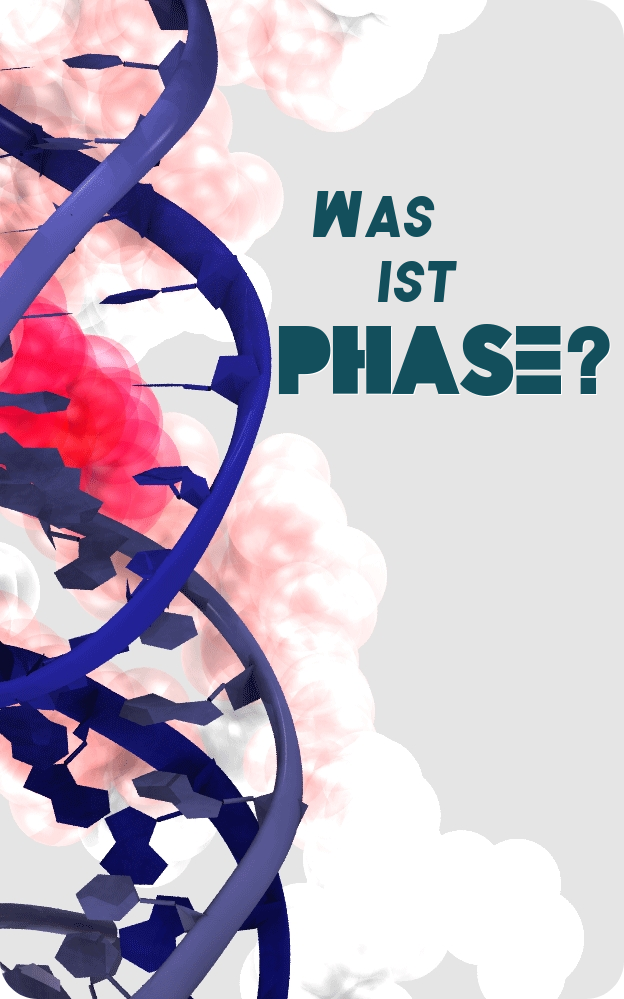
\includegraphics[width=.9\linewidth]{back}
	};
\end{tikzpicture}
%-----------------------------------
%---------- GREEN DECK -------------
%-----------------------------------
%
%-------Prophase
%
\begin{tikzpicture}
	\draw[rounded corners=0.2cm] (0,0) rectangle (\cardwidth,\cardheight);
	\fill[lightgreen,rounded corners=0.1cm] (\strippadding,\strippadding) rectangle (\strippadding+\stripwidth,\cardheight-\strippadding) node[rotate=90,above left,black,font=\large] {FACHBEGRIFF\hspace{3pt}  \rotatebox[origin=c]{-90}{\faIcon{info}}};
	\node[text width=(\cardwidth-\strippadding-\stripwidth-2*\textpadding-0.3)*1cm,below right] at (\strippadding+\stripwidth+\textpadding,\cardheight-\textpadding) {
		{\Large  }\\
		\vspace{0.8cm}
		{\Large Prophase}\\
		\vspace{0.5 cm}
		{\footnotesize aus dem Griechischen: $ \pi\rho $\'{o} \textit{(pr\'{o})}: ,,vor'' \\ $ \varphi \acute{\alpha}\sigma\iota\varsigma$ \textit{(ph\'{a}sis)}: ,,Phase''\\ }
			\vspace{0.1cm}
		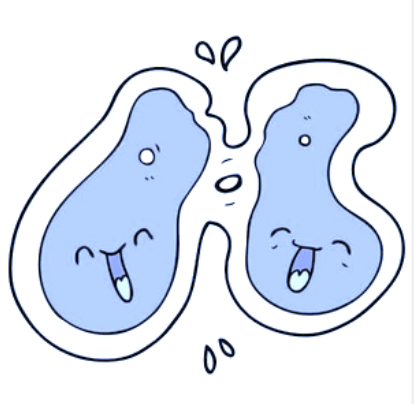
\includegraphics[width=\linewidth]{g/cute5}	
	};
\end{tikzpicture}\hspace{1pt}
%-------Metaphase
\begin{tikzpicture}
	\draw[rounded corners=0.2cm] (0,0) rectangle (\cardwidth,\cardheight);
	\fill[lightgreen,rounded corners=0.1cm] (\strippadding,\strippadding) rectangle (\strippadding+\stripwidth,\cardheight-\strippadding) node[rotate=90,above left,black,font=\large] {FACHBEGRIFF\hspace{3pt}  \rotatebox[origin=c]{-90}{\faIcon{info}}};
	\node[text width=(\cardwidth-\strippadding-\stripwidth-2*\textpadding-0.3)*1cm,below right] at (\strippadding+\stripwidth+\textpadding,\cardheight-\textpadding) {
		{\Large  }\\
		\vspace{0.8cm}
		{\Large Metaphase}\\
		\vspace{0.5 cm}
		{\footnotesize aus dem Griechischen: $\mu\epsilon\tau\acute{\alpha} $ \textit{(met\'{a})}: ,,nachdem'', $ \varphi \acute{\alpha}\sigma\iota\varsigma$ \textit{(ph\'{a}sis)}: ,,Phase''\\ }
		\vspace{0.1cm}
		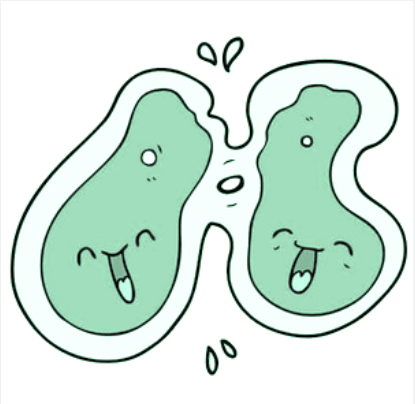
\includegraphics[width=\linewidth]{g/cute2}	
	};
\end{tikzpicture}\hspace{1pt}
%-------Anaphase
\begin{tikzpicture}
\draw[rounded corners=0.2cm] (0,0) rectangle (\cardwidth,\cardheight);
\fill[lightgreen,rounded corners=0.1cm] (\strippadding,\strippadding) rectangle (\strippadding+\stripwidth,\cardheight-\strippadding) node[rotate=90,above left,black,font=\large] {FACHBEGRIFF\hspace{3pt}  \rotatebox[origin=c]{-90}{\faIcon{info}}};
\node[text width=(\cardwidth-\strippadding-\stripwidth-2*\textpadding-0.3)*1cm,below right] at (\strippadding+\stripwidth+\textpadding,\cardheight-\textpadding) {
	{\Large  }\\
	\vspace{0.8cm}
	{\Large Anaphase}\\
	\vspace{0.5 cm}
	{\footnotesize aus dem Griechischen: $ \grave{\alpha}\nu \acute{\alpha}$ \textit{(an\'{a})}: ,,hinauf''\\ $ \varphi \acute{\alpha}\sigma\iota\varsigma$ \textit{(ph\'{a}sis)}: ,,Phase''\\ }
	\vspace{0.1cm}
	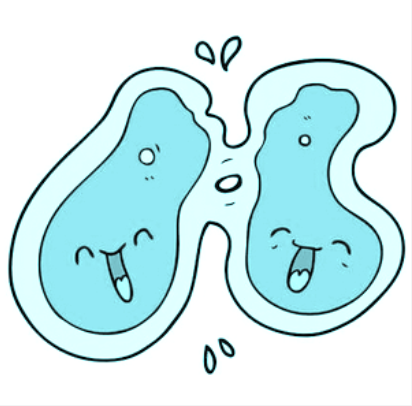
\includegraphics[width=\linewidth]{g/cute3}	
};
\end{tikzpicture}\hspace{1pt}
%-------Telophase
\begin{tikzpicture}
\draw[rounded corners=0.2cm] (0,0) rectangle (\cardwidth,\cardheight);
\fill[lightgreen,rounded corners=0.1cm] (\strippadding,\strippadding) rectangle (\strippadding+\stripwidth,\cardheight-\strippadding) node[rotate=90,above left,black,font=\large] {FACHBEGRIFF\hspace{3pt}  \rotatebox[origin=c]{-90}{\faIcon{info}}};
\node[text width=(\cardwidth-\strippadding-\stripwidth-2*\textpadding-0.3)*1cm,below right] at (\strippadding+\stripwidth+\textpadding,\cardheight-\textpadding) {
	{\Large  }\\
	\vspace{0.8cm}
	{\Large Telophase}\\
	\vspace{0.5 cm}
	{\footnotesize aus dem Griechischen: $\tau\acute{\varepsilon}\lambda o \varsigma$ \textit{(t\'{e}los)}: ,,Ende''\\ $ \varphi \acute{\alpha}\sigma\iota\varsigma$ \textit{(ph\'{a}sis)} :,,Phase''\\ }
	\vspace{0.1cm}
	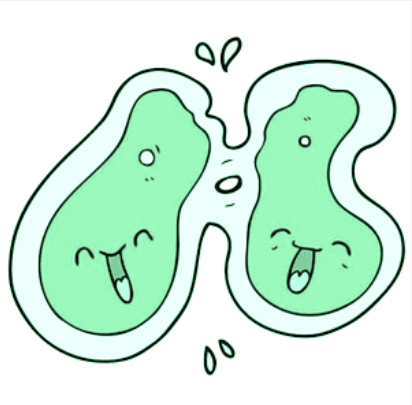
\includegraphics[width=\linewidth]{g/cute4}	
};
\end{tikzpicture}

%-------Cytokinese
\begin{tikzpicture}
	\draw[rounded corners=0.2cm] (0,0) rectangle (\cardwidth,\cardheight);
	\fill[lightgreen,rounded corners=0.1cm] (\strippadding,\strippadding) rectangle (\strippadding+\stripwidth,\cardheight-\strippadding) node[rotate=90,above left,black,font=\large] {FACHBEGRIFF\hspace{3pt}  \rotatebox[origin=c]{-90}{\faIcon{info}}};
	\node[text width=(\cardwidth-\strippadding-\stripwidth-2*\textpadding-0.3)*1cm,below right] at (\strippadding+\stripwidth+\textpadding,\cardheight-\textpadding) {
		{\Large  }\\
		\vspace{0.8cm}
		{\Large Cytokinese}\\
		\vspace{0.5 cm}
		{\footnotesize aus dem Griechischen: $ \kappa\acute{\nu}\tau o\varsigma $ \textit{(k\'{y}tos)}: ,,Zelle''\\ $\kappa\acute{\iota}\nu\eta\sigma\iota\varsigma $ \textit{(k\'{i}nesis)}: ,,Bewegung''\\ }
		\vspace{0cm}
		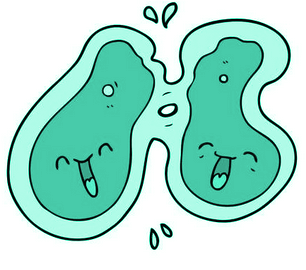
\includegraphics[width=\linewidth]{g/cute1}	
	};
\end{tikzpicture}\hspace{1pt}
%-------Interphase: G1
\begin{tikzpicture}
\draw[rounded corners=0.2cm] (0,0) rectangle (\cardwidth,\cardheight);
\fill[lightgreen,rounded corners=0.1cm] (\strippadding,\strippadding) rectangle (\strippadding+\stripwidth,\cardheight-\strippadding) node[rotate=90,above left,black,font=\large] {FACHBEGRIFF\hspace{3pt}  \rotatebox[origin=c]{-90}{\faIcon{info}}};
\node[text width=(\cardwidth-\strippadding-\stripwidth-2*\textpadding-0.3)*1cm,below right] at (\strippadding+\stripwidth+\textpadding,\cardheight-\textpadding) {
	{\Large  }\\
	\vspace{0.8cm}
	{\Large Interphase: G1}\\
	\vspace{0.5 cm}
	{\footnotesize Inter: ,,zwischen'' (lat.)\\$ \varphi \acute{\alpha}\sigma\iota\varsigma$ \textit{(ph\'{a}sis)} :,,Phase'' (griech.)\\
	G1: ,,Gap 1'' (engl.) \\ }
	\vspace{0.1cm}
	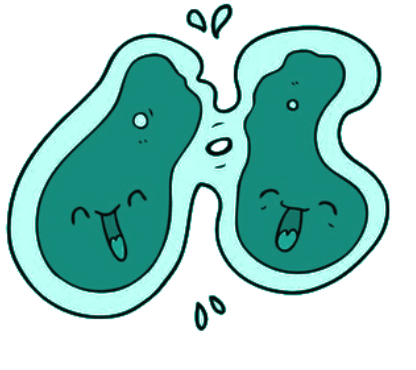
\includegraphics[width=\linewidth]{g/cute9}	
};
\end{tikzpicture}\hspace{1pt}
%------Interphase: S
\begin{tikzpicture}
\draw[rounded corners=0.2cm] (0,0) rectangle (\cardwidth,\cardheight);
\fill[lightgreen,rounded corners=0.1cm] (\strippadding,\strippadding) rectangle (\strippadding+\stripwidth,\cardheight-\strippadding) node[rotate=90,above left,black,font=\large] {FACHBEGRIFF\hspace{3pt}  \rotatebox[origin=c]{-90}{\faIcon{info}}};
\node[text width=(\cardwidth-\strippadding-\stripwidth-2*\textpadding-0.3)*1cm,below right] at (\strippadding+\stripwidth+\textpadding,\cardheight-\textpadding) {
	{\Large  }\\
	\vspace{0.8cm}
	{\Large Interphase: S}\\
	\vspace{0.5 cm}
	{\footnotesize  Inter: ,,zwischen'' (lat.)\\$ \varphi \acute{\alpha}\sigma\iota\varsigma$ \textit{(ph\'{a}sis)} :,,Phase'' (griech.)\\
		S: ,,Synthese'' \\ }
	\vspace{0.1cm}
	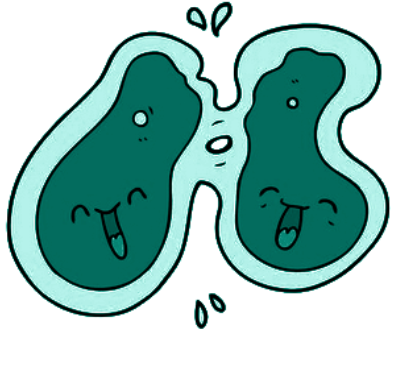
\includegraphics[width=\linewidth]{g/cute8}	
};
\end{tikzpicture}\hspace{1pt}
%-------Interphase: G2
\begin{tikzpicture}
	\draw[rounded corners=0.2cm] (0,0) rectangle (\cardwidth,\cardheight);
	\fill[lightgreen,rounded corners=0.1cm] (\strippadding,\strippadding) rectangle (\strippadding+\stripwidth,\cardheight-\strippadding) node[rotate=90,above left,black,font=\large] {FACHBEGRIFF\hspace{3pt}  \rotatebox[origin=c]{-90}{\faIcon{info}}};
	\node[text width=(\cardwidth-\strippadding-\stripwidth-2*\textpadding-0.3)*1cm,below right] at (\strippadding+\stripwidth+\textpadding,\cardheight-\textpadding) {
		{\Large  }\\
		\vspace{0.8cm}
		{\Large Interphase: G2}\\
		\vspace{0.5 cm}
		{\footnotesize  Inter: ,,zwischen'' (lat.)\\$ \varphi \acute{\alpha}\sigma\iota\varsigma$ \textit{(ph\'{a}sis)} :,,Phase'' (griech.)\\
			G2: ,,Gap 2'' (engl.) \\ }
		\vspace{0.1cm}
		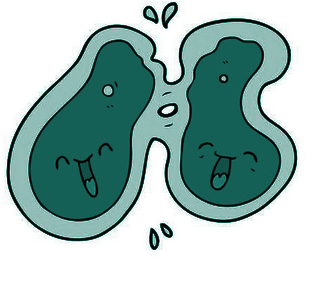
\includegraphics[width=\linewidth]{g/cute7}	
	};
\end{tikzpicture}

%------------------------------------
%----------- ANLEITUNG --------------
%------------------------------------
\begin{tikzpicture}
	\draw[rounded corners=0.2cm] (0,0) rectangle (20 cm,8.5cm);
	\node[text width=(20.5-0.3)*1cm,below right] at (0,\cardheight+\textpadding) {
		{\Large  }\\
		\vspace{-0.25cm}
		\hspace{0.28 cm}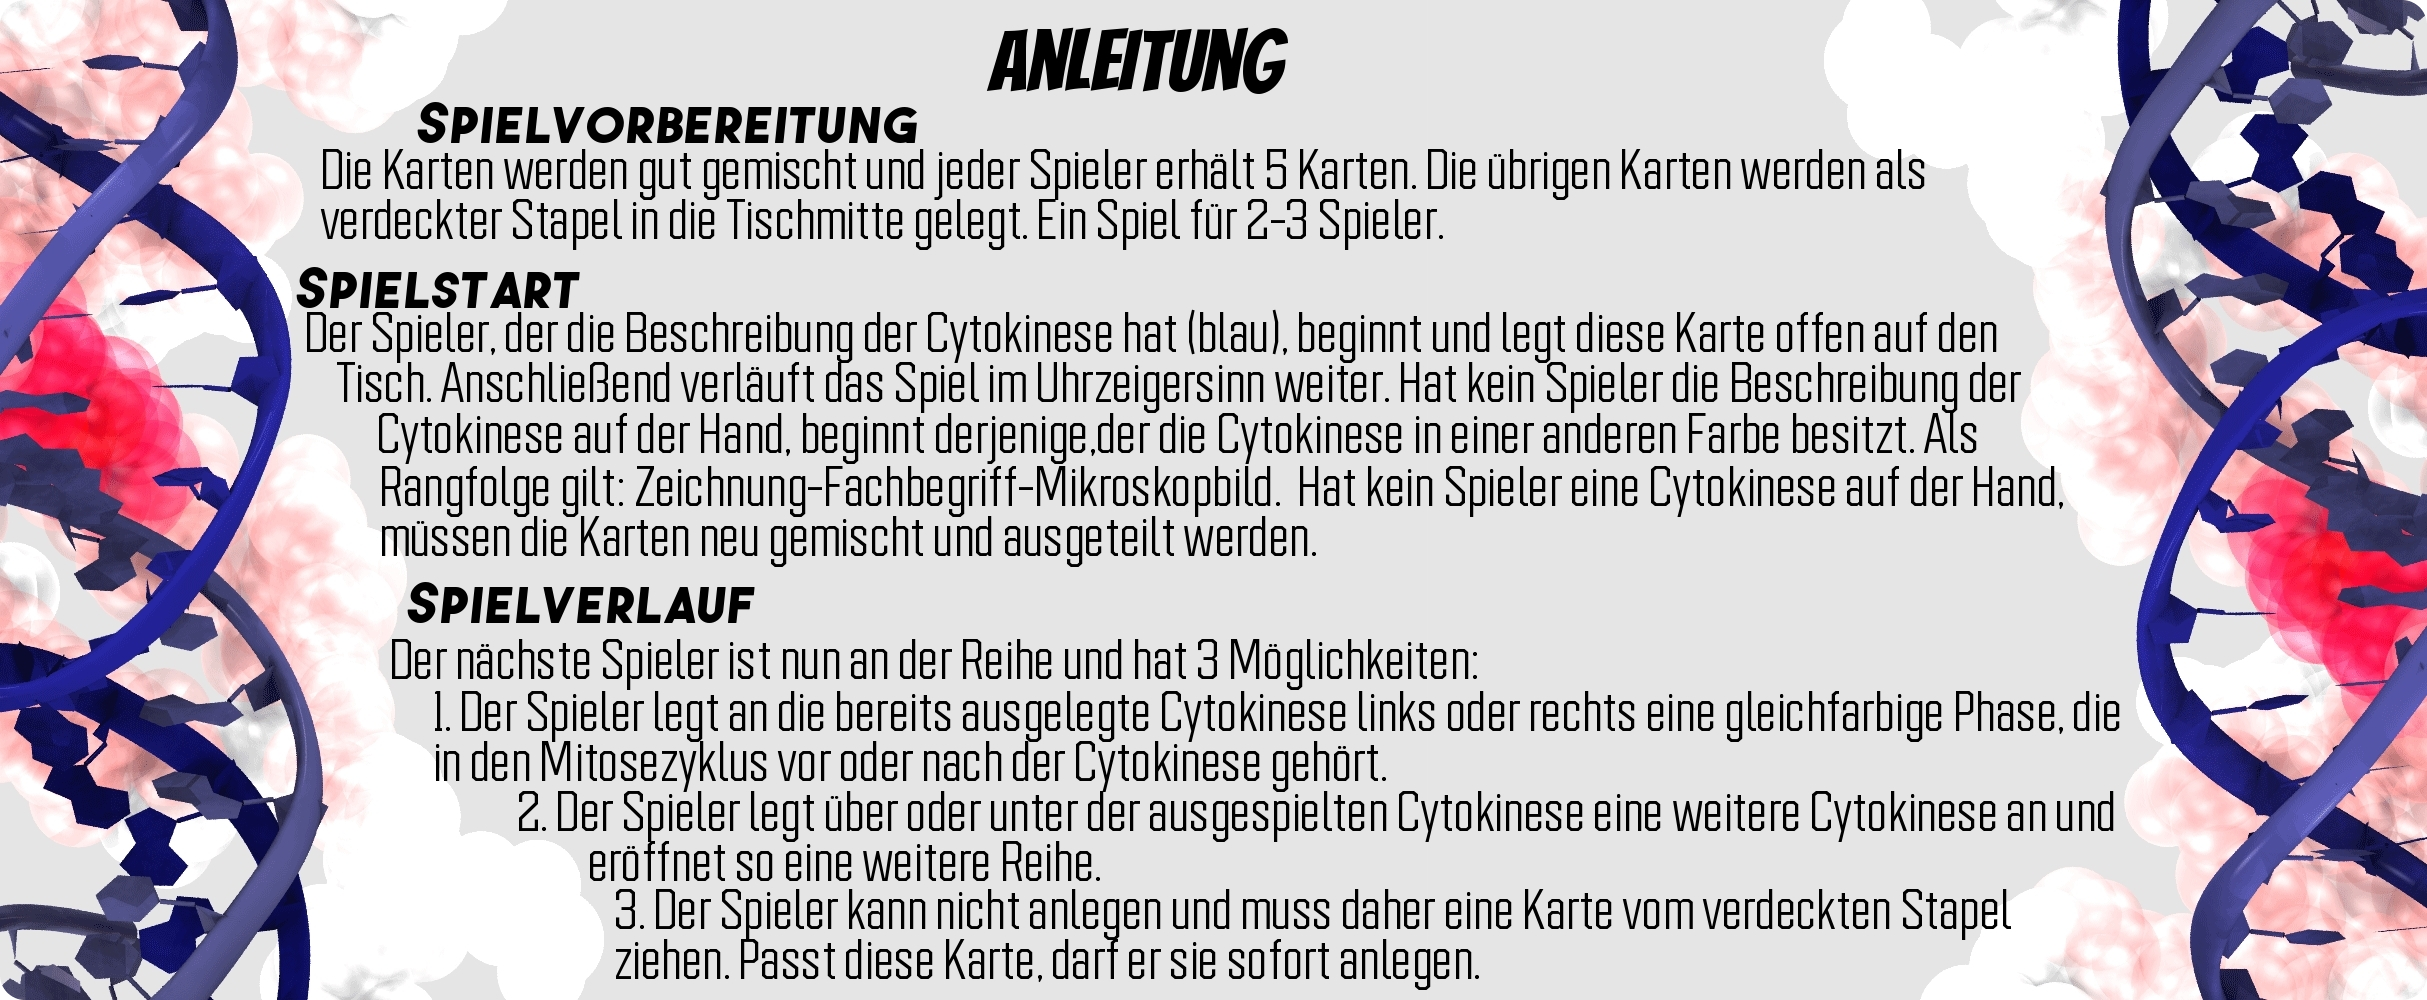
\includegraphics[width=0.95\linewidth]{rule/rule_front}
	};
\end{tikzpicture}
\newpage
%-----------------------------------
%---------- BACK SIDE  -------------
%-----------------------------------
\begin{tikzpicture}
	\draw[rounded corners=0.2cm] (0,0) rectangle (\cardwidth,\cardheight);
	\node[text width=(\cardwidth-0.3)*1cm,below right] at (0,\cardheight+\textpadding) {
		{\Large  }\\
		\vspace{0.3cm}
		\hspace{3pt}\includegraphics[width=0.95\linewidth]{back}
	};
\end{tikzpicture}\hspace{1pt}
\begin{tikzpicture}
	\draw[rounded corners=0.2cm] (0,0) rectangle (\cardwidth,\cardheight);
	\node[text width=(\cardwidth-0.3)*1cm,below right] at (0,\cardheight+\textpadding) {
		{\Large  }\\
		\vspace{0.3cm}
		\hspace{3pt}\includegraphics[width=0.95\linewidth]{back}
	};
\end{tikzpicture}\hspace{1pt}
\begin{tikzpicture}
	\draw[rounded corners=0.2cm] (0,0) rectangle (\cardwidth,\cardheight);
	\node[text width=(\cardwidth-0.3)*1cm,below right] at (0,\cardheight+\textpadding) {
		{\Large  }\\
		\vspace{0.3cm}
		\hspace{3pt}\includegraphics[width=0.95\linewidth]{back}
	};
\end{tikzpicture}\hspace{1pt}
\begin{tikzpicture}
	\draw[rounded corners=0.2cm] (0,0) rectangle (\cardwidth,\cardheight);
	\node[text width=(\cardwidth)*1cm,below right] at (0,\cardheight+\textpadding) {
		{\Large  }\\
		\vspace{0.3cm}
		\hspace{3pt}\includegraphics[width=.9\linewidth]{back}
	};
\end{tikzpicture}

\begin{tikzpicture}
	\draw[rounded corners=0.2cm] (0,0) rectangle (\cardwidth,\cardheight);
	\node[text width=(\cardwidth-0.3)*1cm,below right] at (0,\cardheight+\textpadding) {
		{\Large  }\\
		\vspace{0.3cm}
		\hspace{3pt}\includegraphics[width=0.95\linewidth]{back}
	};
\end{tikzpicture}\hspace{1pt}
\begin{tikzpicture}
	\draw[rounded corners=0.2cm] (0,0) rectangle (\cardwidth,\cardheight);
	\node[text width=(\cardwidth-0.3)*1cm,below right] at (0,\cardheight+\textpadding) {
		{\Large  }\\
		\vspace{0.3cm}
		\hspace{3pt}\includegraphics[width=0.95\linewidth]{back}
	};
\end{tikzpicture}\hspace{1pt}
\begin{tikzpicture}
	\draw[rounded corners=0.2cm] (0,0) rectangle (\cardwidth,\cardheight);
	\node[text width=(\cardwidth-0.3)*1cm,below right] at (0,\cardheight+\textpadding) {
		{\Large  }\\
		\vspace{0.3cm}
		\hspace{3pt}\includegraphics[width=0.95\linewidth]{back}
	};
\end{tikzpicture}\hspace{1pt}
\begin{tikzpicture}
	\draw[rounded corners=0.2cm] (0,0) rectangle (\cardwidth,\cardheight);
	\node[text width=(\cardwidth)*1cm,below right] at (0,\cardheight+\textpadding) {
		{\Large  }\\
		\vspace{0.3cm}
		\hspace{3pt}\includegraphics[width=.9\linewidth]{back}
	};
\end{tikzpicture}\vspace{5pt}
%------------------------------------
%----------- ANLEITUNG --------------
%------------------------------------
\begin{tikzpicture}
	\draw[rounded corners=0.2cm] (0,0) rectangle (20 cm,8.5cm);
	\node[text width=(20.5-0.3)*1cm,below right] at (0,\cardheight+\textpadding) {
		{\Large  }\\
		\vspace{-0.25cm}
		\hspace{0.28 cm}\includegraphics[width=0.95\linewidth]{rule/rule_back}
	};
\end{tikzpicture}

\newpage
%----------------------------
%--------- Lösungen ---------
%----------------------------


\begin{center}
	\begin{huge}
		\noindent Lösung\\
		
	\end{huge}

\noindent \textbf{Hinweis:}
Die Phasen sind zyklisch und werden von links nach rechts gelesen.

	\includegraphics[scale=0.75]{solution/fachbegriff.png} 
	\includegraphics[scale=0.75]{solution/beschreibung.png} 	
	\includegraphics[scale=0.75]{solution/mikroskop.png} 		
	\includegraphics[scale=0.75]{solution/skizze.png}
\end{center}

\end{document}

%
%
%
%-----------------------------------
%---------- SHENANIGANS  -----------
%-----------------------------------
%\begin{tikzpicture}
%	\draw[rounded corners=0.2cm] (0,0) rectangle (\cardwidth,\cardheight);
%	\draw (0,0) node[text width=(\cardwidth)*1cm,below right] at (0,\cardheight+\textpadding) {
%		{\Large  }\\
%		\vspace{0.3cm}
%		\hspace{3pt}\includegraphics[width=.9\linewidth]{werwe}
%	};
%	\draw (\cardwidth/2,\cardheight/2) node[rotate=58]{\Huge \textcolor{black}{Text}};
%\end{tikzpicture}
%




%-----------------------------------
%-----------REFACTORING--------------
%------------------------------------
%


%------------------------------------
%--------SHORTEND COMMANDS ----------
%------------------------------------
%


\newpage

% green card
% arguments [color, title, icon, content]
\newcommand{\customCard}[4]{
	\begin{tikzpicture}
		\draw[rounded corners=0.2cm] (0,0) rectangle (\cardwidth,\cardheight);
		\fill[#1,rounded corners=0.1cm] (\strippadding,\strippadding) rectangle (\strippadding+\stripwidth,\cardheight-\strippadding) node[rotate=90,above left,black,font=\large] {#2\hspace{3pt}  \rotatebox[origin=c]{-90}{#3}};
		\node[text width=(\cardwidth-\strippadding-\stripwidth-2*\textpadding-0.3)*1cm,below right] at (\strippadding+\stripwidth+\textpadding,\cardheight-\textpadding) {#4};
	\end{tikzpicture}
}
\newcommand{\testCard}{\customCard{blue}{Test Card}{\faIcon{search}}{Text Content}}

% pink card
% arguments [image]
\newcommand{\pinkCard}[1]{\customCard
	{pink}
	{UNTER DEM MIKROSKOP}
	{\faIcon{microscope}}
	{{\Large  }\\
		\vspace{0.7cm}
		\includegraphics[width=\linewidth]{#1}}}

% orange card
% arguments [image]
\newcommand{\orangeCard}[1]{\customCard
	{apricot}
	{ZEICHNUNG}
	{\footnotesize\faIcon[regular]{edit}}
	{{\Large  }\\
		\vspace{0.9cm}
		\includegraphics[width=\linewidth]{#1}}}

% blue card
% arguments [text]
\newcommand{\blueCard}[1]{\customCard
	{lightblue}
	{BESCHREIBUNG}
	{\faIcon[regular]{file-alt}}
	{{\Large  }\\
		\vspace{0.6cm}
		{\scriptsize #1}}}

% green card
% arguments [title, text, image]
\newcommand{\greenCard}[3]{\customCard
	{lightgreen}
	{FACHBEGRIFF}
	{\faIcon{info}}
	{{\Large  }\\
		\vspace{0.8cm}
		{\Large Prophase}\\
		\vspace{0.5 cm}
		{\footnotesize #2\\ }
		\vspace{0.1cm}
		\includegraphics[width=\linewidth]{#3}}}

% examples
%\pinkCard{p/interphase}
%\pinkCard{p/prophase}
%\pinkCard{p/prophase2}
%\pinkCard{p/metaphase}
%
%\pinkCard{p/anaphase1}
%\pinkCard{p/anaphase2}
%\pinkCard{p/telophase2}
%\pinkCard{p/cytokinese}
%
%
%\orangeCard{zeichnung}
%\orangeCard{zeichnung}
%
%\blueCard{Lorem ipsum dolor sit amet, consectetur adipisicing elit, sed do eiusmod tempor incididunt ut labore et dolore magna aliqua. Lorem ipsum dolor sit amet, consectetur adipisicing elit. Sed do eiusmod tempor incididunt ut labore et dolore magna aliqua.}
%\blueCard{Super informativer Text über diese Karte.}
%\greenCard{Prophase}{aus dem Griechischen: $ \pi\rho $\'{o} \textit{(pr\'{o})}: ,,vor'' \\ $ \varphi \acute{\alpha}\sigma\iota\varsigma$ \textit{(ph\'{a}sis)}: ,,Phase''}{cute2}
%\greenCard{Test2}{Text mit Erklaerung}{cute5}
